\clearemptydoublepage
\chapter{Trabajo Realizado}
\chaptermark{Trabajo Realizado}

En este capítulo intentaré explicar y mostrar los aspectos generales de las funciones que llegué a desarrollar durante mis prácticas.
Proporcionaré diagramas de datos y algunas imágenes que ayuden a entender la idea que hay detrás de muchas soluciones a los problemas a los que nos enfrentamos como equipo.

La información real del proyecto permanecerá oculta por cuestiones de confidencialidad, pero no afectará a la comprensión del trabajo.

\section{Planeación de Desarrollo}

Mi trabajo se llevó a cabo durante 6 meses de trabajo en el instituto. A modo ilustrativo del tiempo requerido para realizar las tareas asignadas, podemos ver el siguiente diagrama de Gantt.

Cada herramienta desarrollada requiere una adecuada documentación dentro del GitLab del proyecto para poder mantener registro del progreso, de los métodos de programación utilizados y cualquier explicación que pueda ayudar a entender rápidamente qué se realizó.

\begin{figure}[ht]
    \begin{center}
       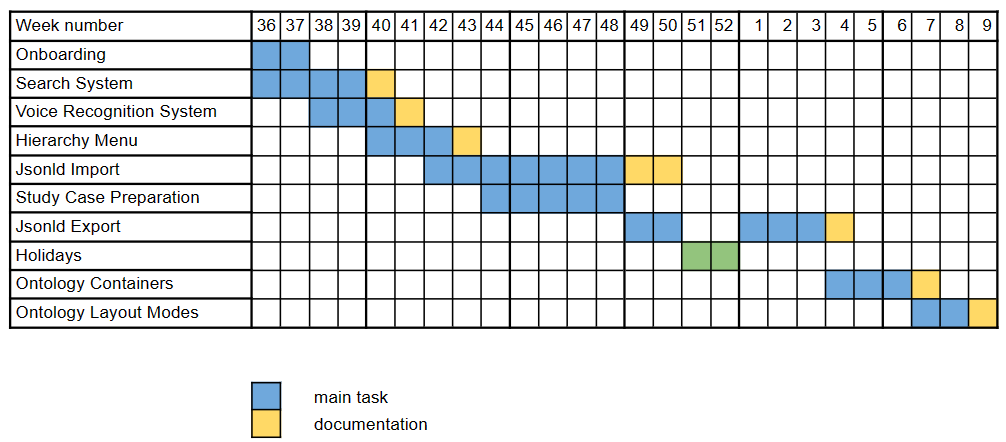
\includegraphics[width=1\linewidth]{chapter2/figures/gantt.png}
    \end{center}
    \caption[Planeacion de Desarrollo en Diagrama de Gantt]
    {\footnotesize Planeacion de Desarrollo en Diagrama de Gantt}
 \end{figure}

 \section{Software de Desarrollo}

El proyecto se desarrolló con Unity (versión 2021.3.23f1). Se trata de una plataforma de desarrollo de juegos potente y versátil que ha revolucionado la forma de crear juegos, desde proyectos independientes hasta grandes éxitos de taquilla. Con Unity, los desarrolladores pueden diseñar, crear e implantar juegos de alta calidad en multitud de plataformas, como dispositivos móviles, consolas y PC. Su interfaz fácil de usar y su amplia biblioteca de recursos lo hacen accesible tanto para los profesionales experimentados como para los recién llegados al desarrollo de juegos.

Uno de los aspectos más atractivos de Unity es su capacidad para facilitar la creación rápida de prototipos y la iteración. Los desarrolladores pueden dar vida rápidamente a sus ideas, probar mecánicas de juego y perfeccionar sus creaciones en tiempo real. Esta agilidad no sólo acelera el proceso de desarrollo, sino que también permite una mayor creatividad y experimentación.

Además, Unity ofrece un vasto ecosistema de activos, plugins y apoyo de la comunidad, lo que permite a los desarrolladores ampliar la funcionalidad de la plataforma y colaborar con otros creadores. Desde activos y scripts prefabricados hasta técnicas avanzadas de renderizado y algoritmos de inteligencia artificial, Unity proporciona una gran cantidad de recursos para agilizar el desarrollo y mejorar la calidad de los juegos.

\subsection{OpenXR}

Para conectar Unity con el casco de realidad virtual, optamos por OpenXR, un estándar abierto que pretende agilizar el desarrollo de aplicaciones de realidad virtual proporcionando una API común para interactuar con el hardware de realidad virtual. Desarrollado por Khronos Group, un consorcio industrial centrado en el desarrollo de estándares abiertos para gráficos y computación paralela, OpenXR pretende abordar la fragmentación del ecosistema de realidad virtual y realidad aumentada permitiendo a los desarrolladores crear aplicaciones compatibles con una amplia gama de dispositivos, plataformas y entornos de ejecución. \cite[]{OpenXR}

\begin{figure}[ht]
   \begin{center}
      
\includegraphics[width=0.4\linewidth]{chapter2/figures/OpenXR_logo.png}
   \end{center}
   \caption[OpenXR logo]
   {\footnotesize OpenXR logo}
\end{figure}

Proporciona un conjunto de API estándar para funciones como el renderizado, el manejo de entradas, el seguimiento y la interacción, lo que permite a los desarrolladores acceder y controlar las capacidades de los dispositivos de hardware de realidad virtual y realidad aumentada de forma coherente e independiente de la plataforma.
Esto fue de enorme relevancia, debido a que en nuestro departamento disponíamos de diferentes headsets para desarrollo y presentaciones, como el HTC Vive Pro, HTC Focus y Meta Quest 2 y 3, por lo que la estandarización fue crucial para la mejora consistente en nuestro proyecto.

\subsection{XR Interaction Toolkit}

Otro elemento central de este proyecto fue el uso del \textit{XR Interaction Toolkit} de Unity, que permite todo tipo de interacciones entre el jugador y el entorno.

El paquete XR Interaction Toolkit es un sistema de interacción de alto nivel basado en componentes para crear experiencias de realidad virtual y realidad aumentada. Proporciona un marco que hace que las interacciones 3D y de interfaz de usuario estén disponibles a partir de eventos de entrada de Unity. El núcleo de este sistema es un conjunto de componentes base \textit{Interactor} e \textit{Interactable}, y un \textit{Interaction Manager} que une estos dos tipos de componentes. \cite[]{XRInteraction}

Luego daré algunos ejemplos de interacciones posibles gracias a este kit de desarrollo.

\section{Visualizador de Ontologías}

Esta aplicación tiene objetivos y estructura muy concretos. En primer lugar, desarrollar herramientas utilizando el formato utilizado por Gaia-X, por lo que debemos incorporar un método para leer los archivos provenientes de este proyecto y para funcionar en conjunto con las otras opciones de software actuales.
Segundo, enfocarnos en tareas estrictamente de visualización de ontologías y no tanto de creación o \textit{debugging}. Este último punto nos determina el tipo de herramientas a priorizar, como pueden ser métodos de filtrado de clases,
búsqueda, comparación de propiedades, manipulación de la apariencia de las ontologías, etc. Más adelante, una vez tengamos este punto cubierto, veremos qué podemos desarrollar para la edición de una ontología. Mientras tanto, debemos
asegurarnos de poder incorporar nuestra aplicación al conjunto de software disponible y así utilizarla en conjunto con las opciones dedicadas a otras tareas.

Antes de explicar las herramientas que desarrollé, es conveniente mostrar cómo se compone la escena y cuáles son los \textit{game objects} que van a estar interactuando.

En nuestro proyecto, decidimos representar una clase utilizando una burbuja. Esta se conecta a otras semejantes a través de flechas de dos colores según el tipo de conexión:

\begin{itemize}
   \item Herencia: en el que se especifica que una clase es subclase de otra de mayor jerarquía. (conexión naranja)
   \item Relación específica: una conexión que incluye una etiqueta de texto para especificar de qué manera se conectan dichas clases. (conexión azul) 
\end{itemize}

\begin{figure}[ht]
   \centering
   \begin{subfigure}{0.3\textwidth}
       \centering
       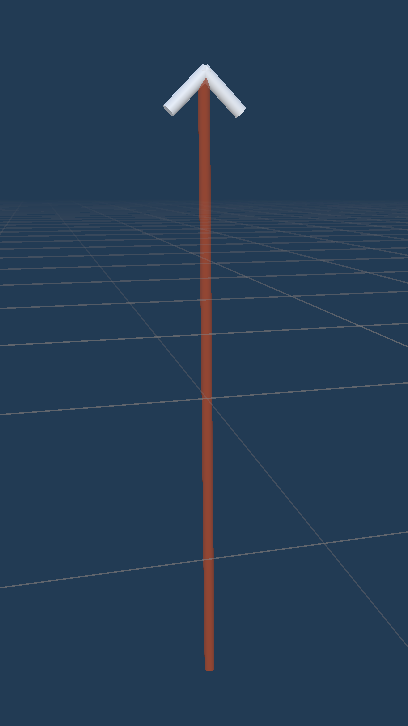
\includegraphics[height=\textwidth]{chapter2/figures/subclass.png}
       \caption{Subclase}
   \end{subfigure}
   \hfill
   \begin{subfigure}{0.3\textwidth}
       \centering
       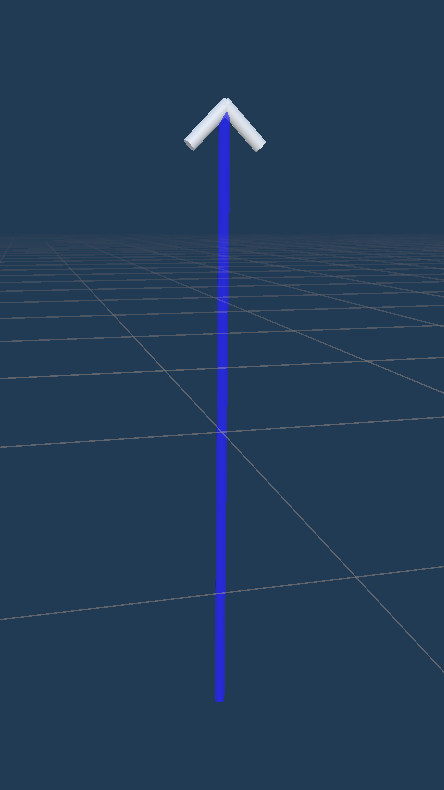
\includegraphics[height=\textwidth]{chapter2/figures/hasconnection.png}
       \caption{Conexión}
   \end{subfigure}
   \hfill
   \begin{subfigure}{0.3\textwidth}
       \centering
       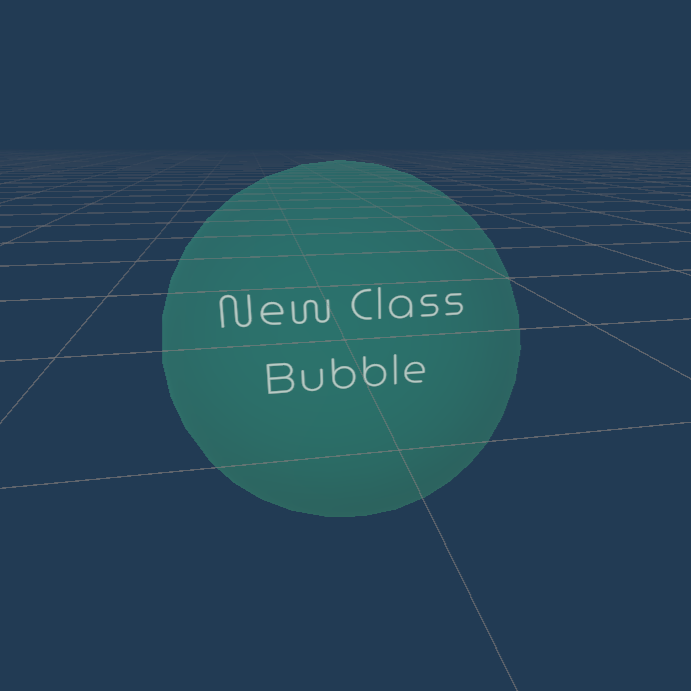
\includegraphics[height=\textwidth]{chapter2/figures/newbubble.png}
       \caption{Nueva burbuja}
   \end{subfigure}
   \caption{Prefabs de conectores y burbuja}
\end{figure}

Un objeto burbuja que representa una clase tiene una serie de variables y listas que le dan identidad única y le brindan la información necesaria para construir el mapa de conexiones.

\begin{enumerate}
   \item UniqueID: id numérico que representa al objeto dentro de la simulación.
   \item Nombre de la clase.
   \item Nombre de la ontología a la que pertenece.
   \item Lista de burbujas con destino de conexión a la burbuja actual (ownedByBubblesList).
   \item Lista de burbujas con origen de conexión en la burbuja actual (hasBubblesIDsList).
   \item Lista de burbujas de las que hereda la burbuja actual (inheritedBubblesList).
   \item Lista de burbujas a las que hereda la burbuja actual (inheritingBubblesIDsList).
   \item Lista de comentarios o propiedades de la clase (elementPropertyValues).
\end{enumerate}

Los primeros 3 items son necesarios para construir la clase, es decir, deben contener valores. Las listas pueden estar vacías, lo cual significa que la clase no tiene conexiones.

\lstinputlisting[caption={Información que contiene cada Burbuja}, label=lst:csharp, linerange={47-70}]{appendix/codes/Bubble.cs}

La escena desarrollada se ve como en la Figura 2.4. Aquí podemos observar, desde el punto de vista del usuario, como se enfrentaría a un grupo de clases provenientes de 4 ontologías diferentes.

\begin{figure}[ht]
   \begin{center}
      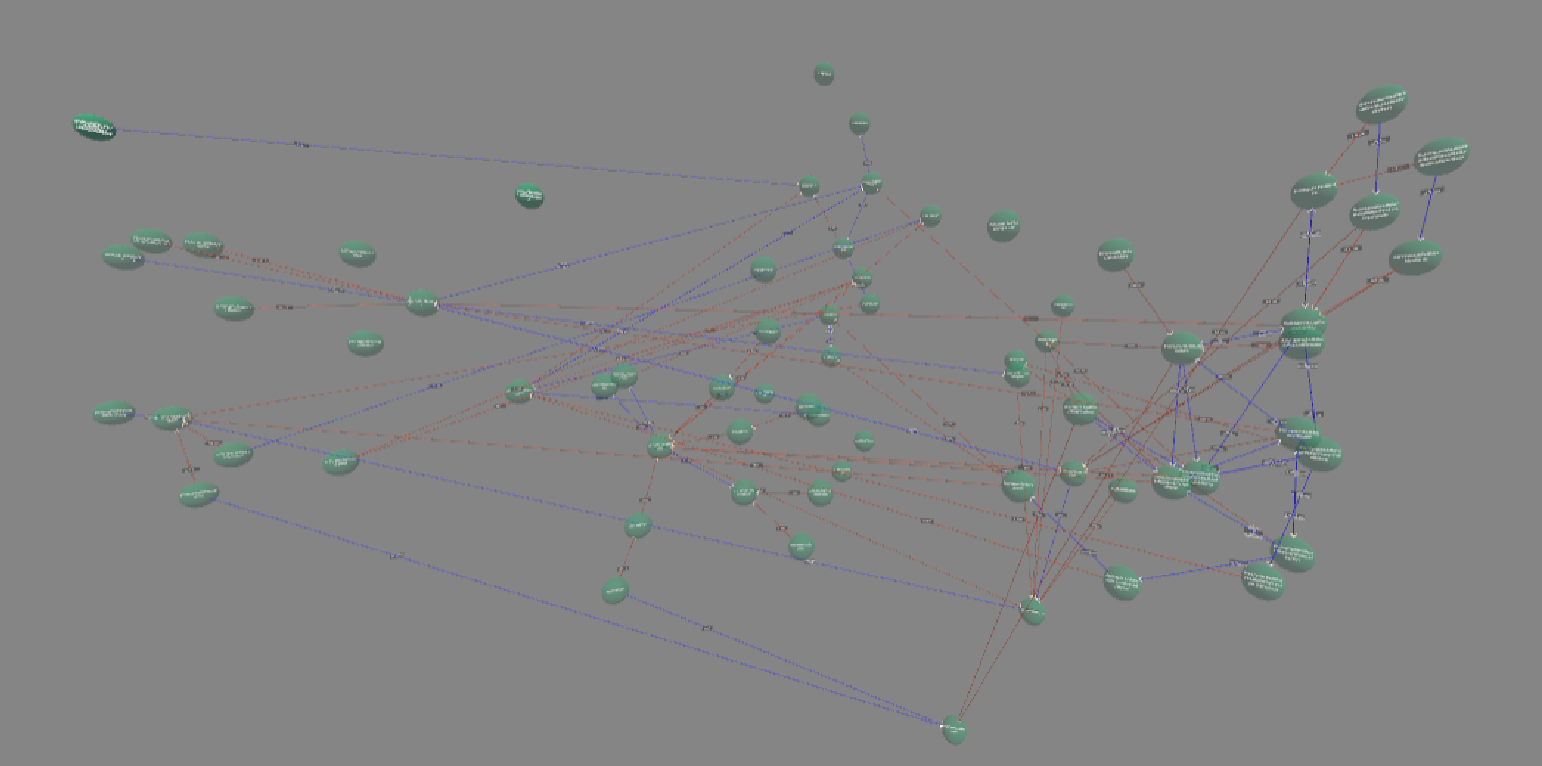
\includegraphics[width=0.8\linewidth]{chapter2/figures/ontology_project.png}
   \end{center}
   \caption[Escena desarrollada]
   {\footnotesize Escena desarrollada}
\end{figure}

El usuario cuenta con 2 controles de mano para relacionarse con la simulación. La mano izquierda está vinculada a un menú con paneles de información y botones para lanzar tareas. La mano derecha, en cambio, proyecta un puntero láser llamado \textit{Raycast} que realiza cálculos de intersección con los objetos presentes en la escena (Ver Figura 2.5). Así, el usuario puede trabajar con su mano derecha interactuando con las burbujas, o posicionar el menú con la mano izquierda y seleccionar con el puntero.

\begin{figure}[ht]
   \begin{center}
      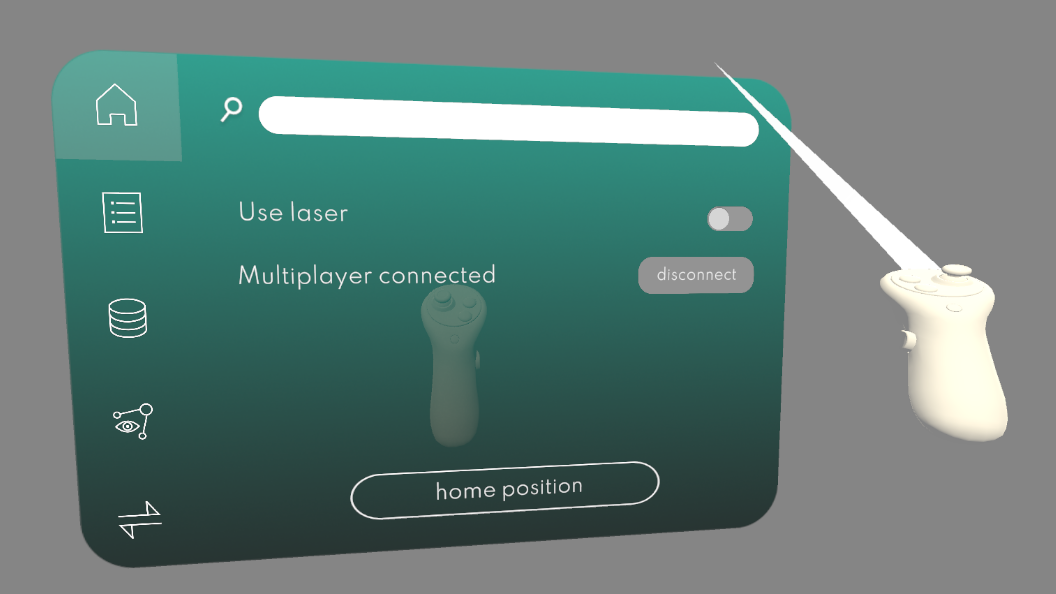
\includegraphics[width=0.6\linewidth]{chapter2/figures/controllers.png}
   \end{center}
   \caption[Menú y puntero de los controladores]
   {\footnotesize Menú y puntero de los controladores}
\end{figure}

El raycast del controlador de la mano derecha puede generar interacciones de diferente tipo según la combinación de botones que se utilice al reconocer un objeto intersectado por el rayo. Con el puntero raycast, manteniendo el botón del dedo índice (normalmente llamado \textit{Trigger}) presionado mientras apuntamos a una burbuja, podemos moverla en el espacio como queramos. Ese mismo puntero también nos permite teletransportarnos a dicha burbuja si movemos el joystick hacia adelante mientras apuntarmos en vez de presionar el trigger. Las interacciones con el menú se realizan con el mismo puntero y seleccionando los botones que queramos utilizando el mismo trigger.

\begin{figure}[ht]
   \centering
   \begin{subfigure}{0.45\textwidth}
       \centering
       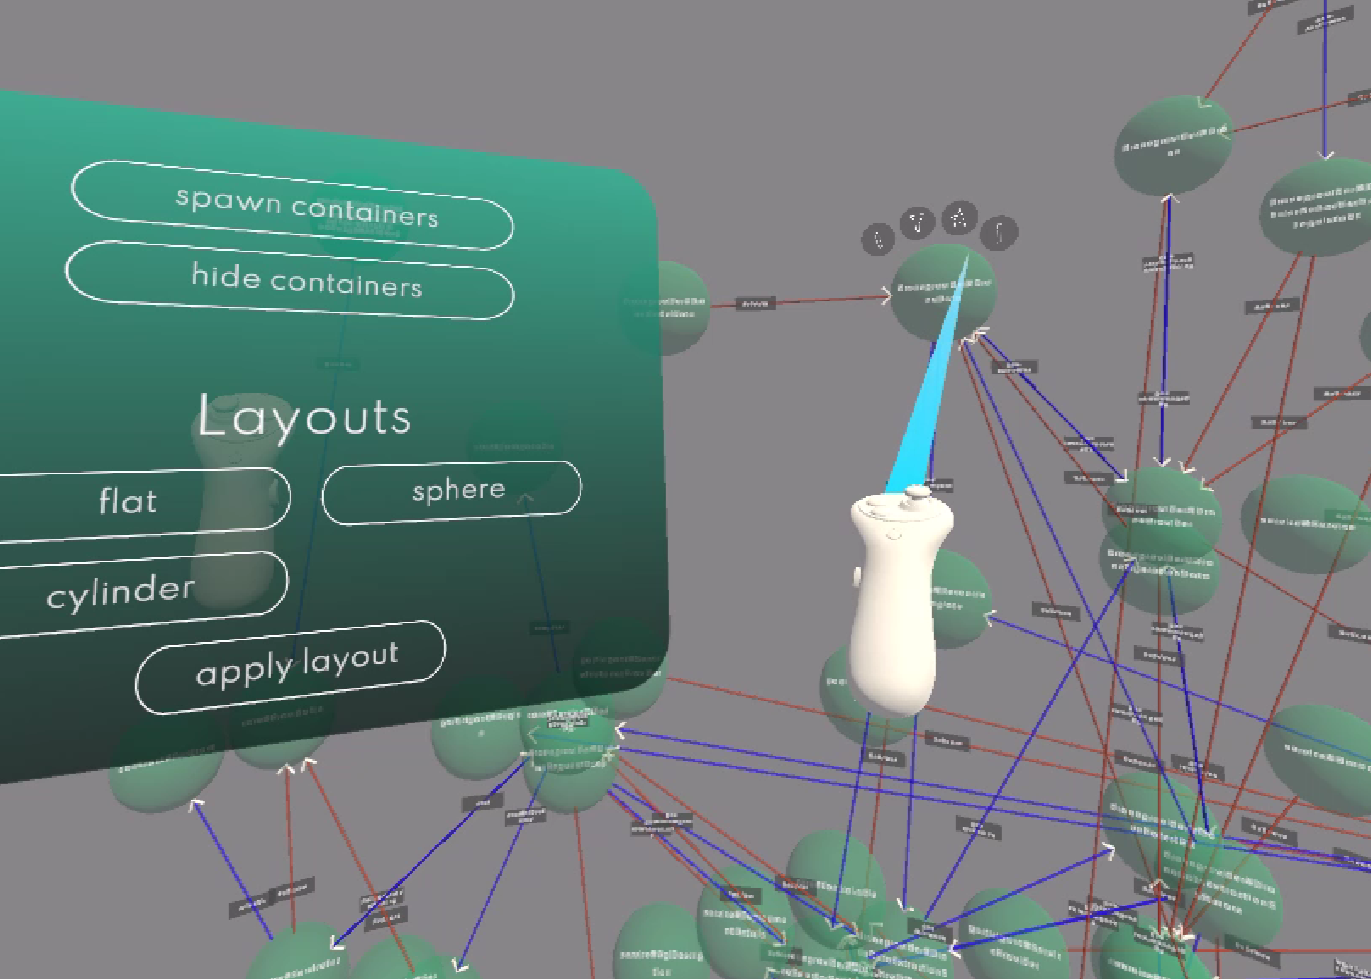
\includegraphics[width=\textwidth]{chapter2/figures/raycast.png}
       \caption{Puntero Raycast}
   \end{subfigure}
   \hfill
   \begin{subfigure}{0.45\textwidth}
       \centering
       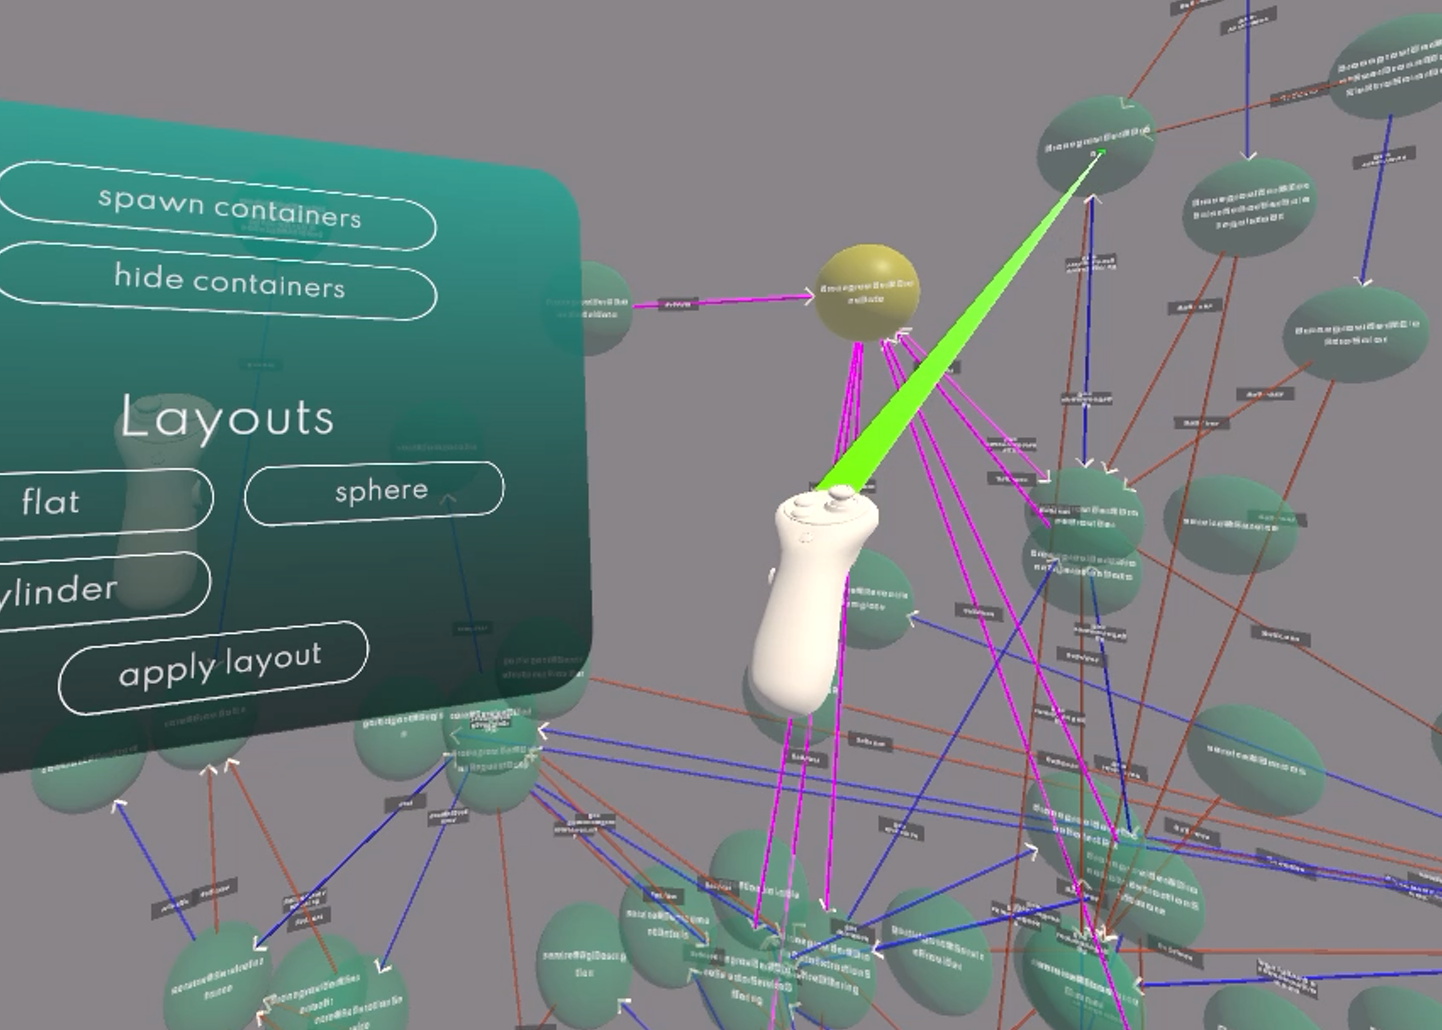
\includegraphics[width=\textwidth]{chapter2/figures/teleport.png}
       \caption{Teletransportación}
   \end{subfigure}
   \begin{subfigure}{0.45\textwidth}
       \centering
       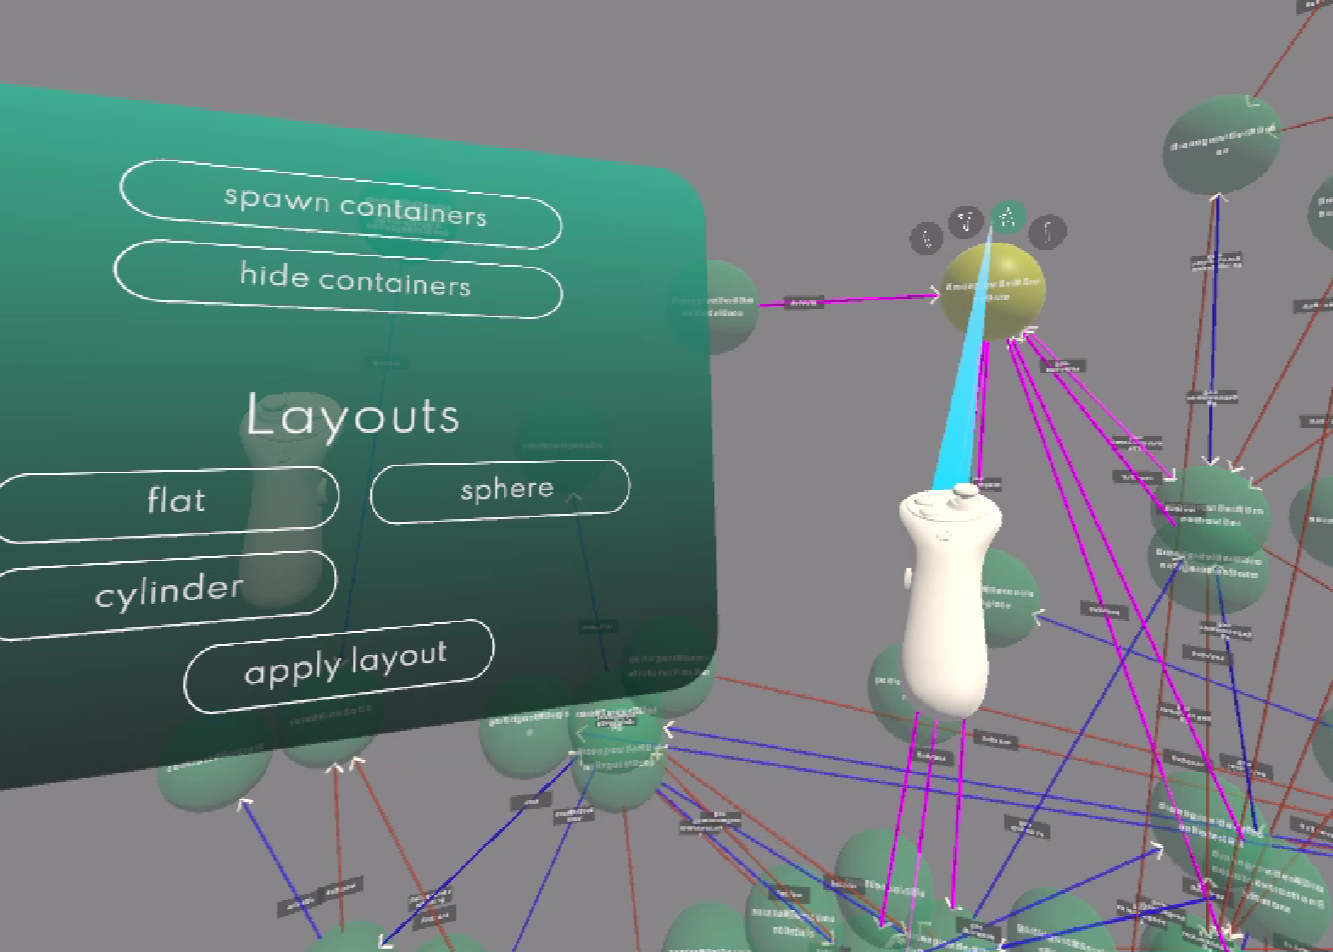
\includegraphics[width=\textwidth]{chapter2/figures/highlight.png}
       \caption{Interacciones con UI}
   \end{subfigure}
   \hfill
   \begin{subfigure}{0.45\textwidth}
      \centering
      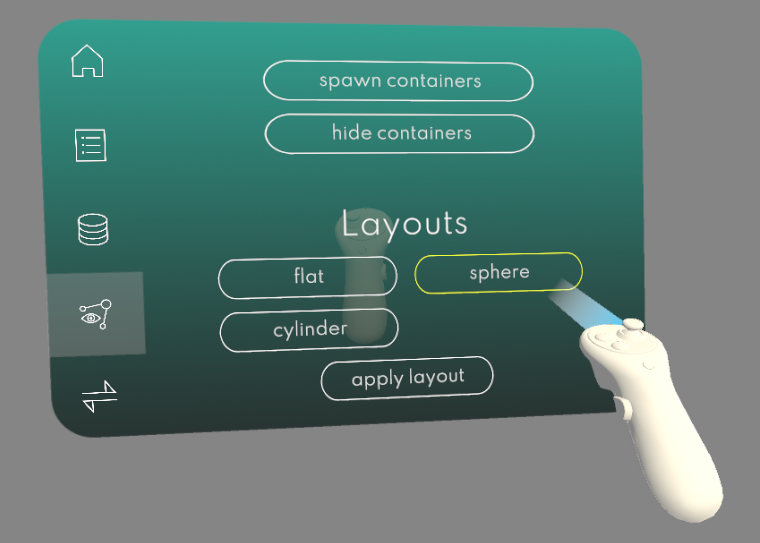
\includegraphics[width=\textwidth]{chapter2/figures/menu_interaction.png}
      \caption{Interacciones con el menú}
  \end{subfigure}
  \caption{Interaccioes del Toolkit}
\end{figure}

\section{Herramientas pre-existentes}

En esta sección voy a mostrar las herramientas que ya existían en la escena en el momento de mi comienzo en el proyecto. Es importante explicarlas rápidamente ya que parte de mi tarea fue integrar mis funciones a lo ya existente, al igual que solucionar los posibles errores que surgieran de aumentar las interacciones entre los códigos.

Al apuntarle a una burbuja, aparece sobre ella un menú con distintos botones asociados a las funciones que veremos en las siguientes páginas.

\subsection{Filtrar por conexiones}

Esta herramienta es de las mas útiles en nuestro visualizador ya que se encarga de mostrar sólo las burbujas directamente conectadas a la burbuja que seleccionemos. Esto se hace apagando el componente físico de todas las burbujas de la escena excepto la burbuja seleccionada y sus conexiones. Así, podremos visualizar muy rápidamente, filtrando una gran cantidad de objetos, una burbuja deseada y sus relaciones.

\begin{figure}[ht]
   \centering
   \begin{subfigure}{0.45\textwidth}
       \centering
       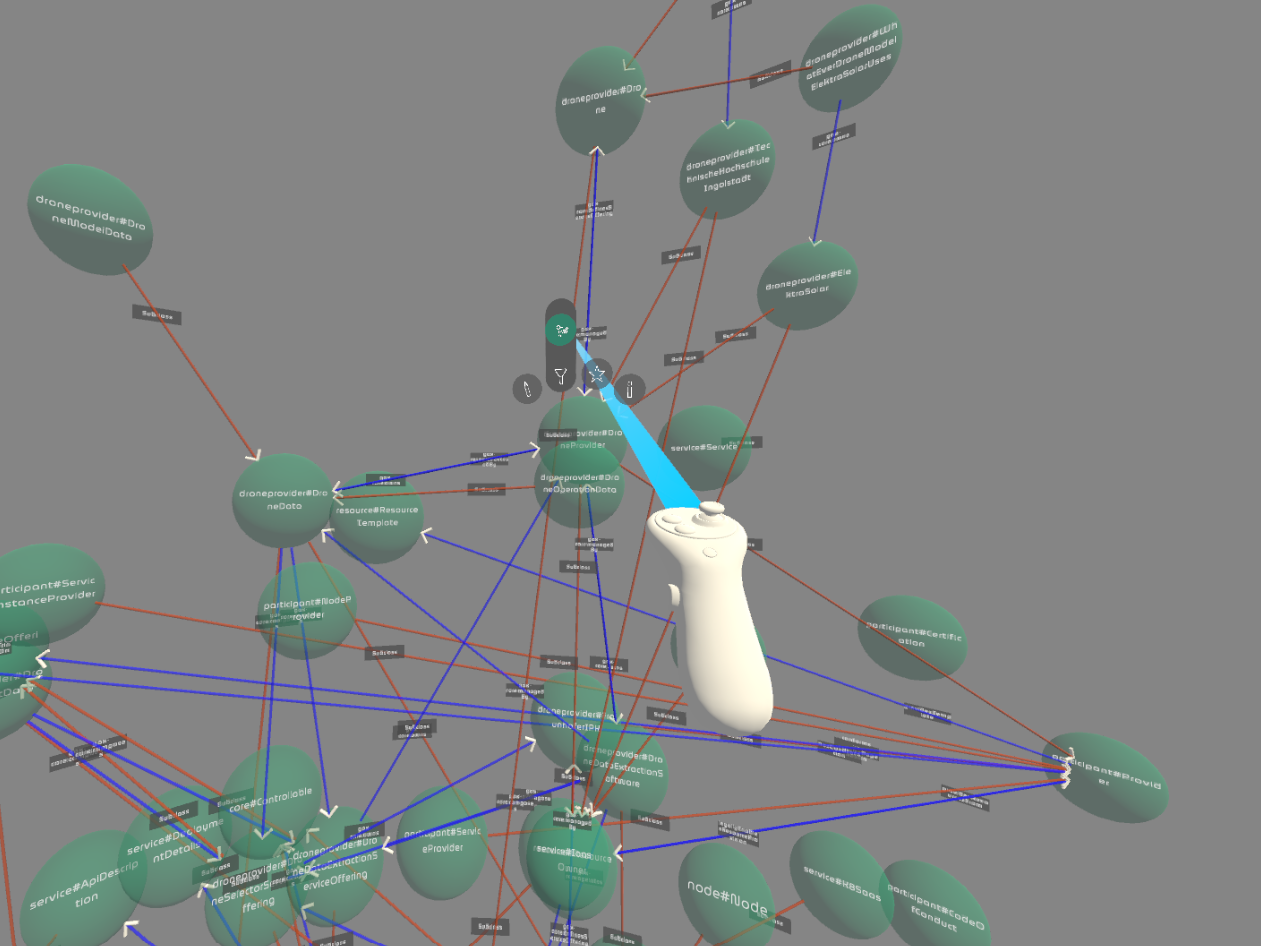
\includegraphics[width=\textwidth]{chapter2/figures/prefilter.png}
       \caption{Fragmento de escena antes de filtrar}
   \end{subfigure}
   \hfill
   \begin{subfigure}{0.45\textwidth}
       \centering
       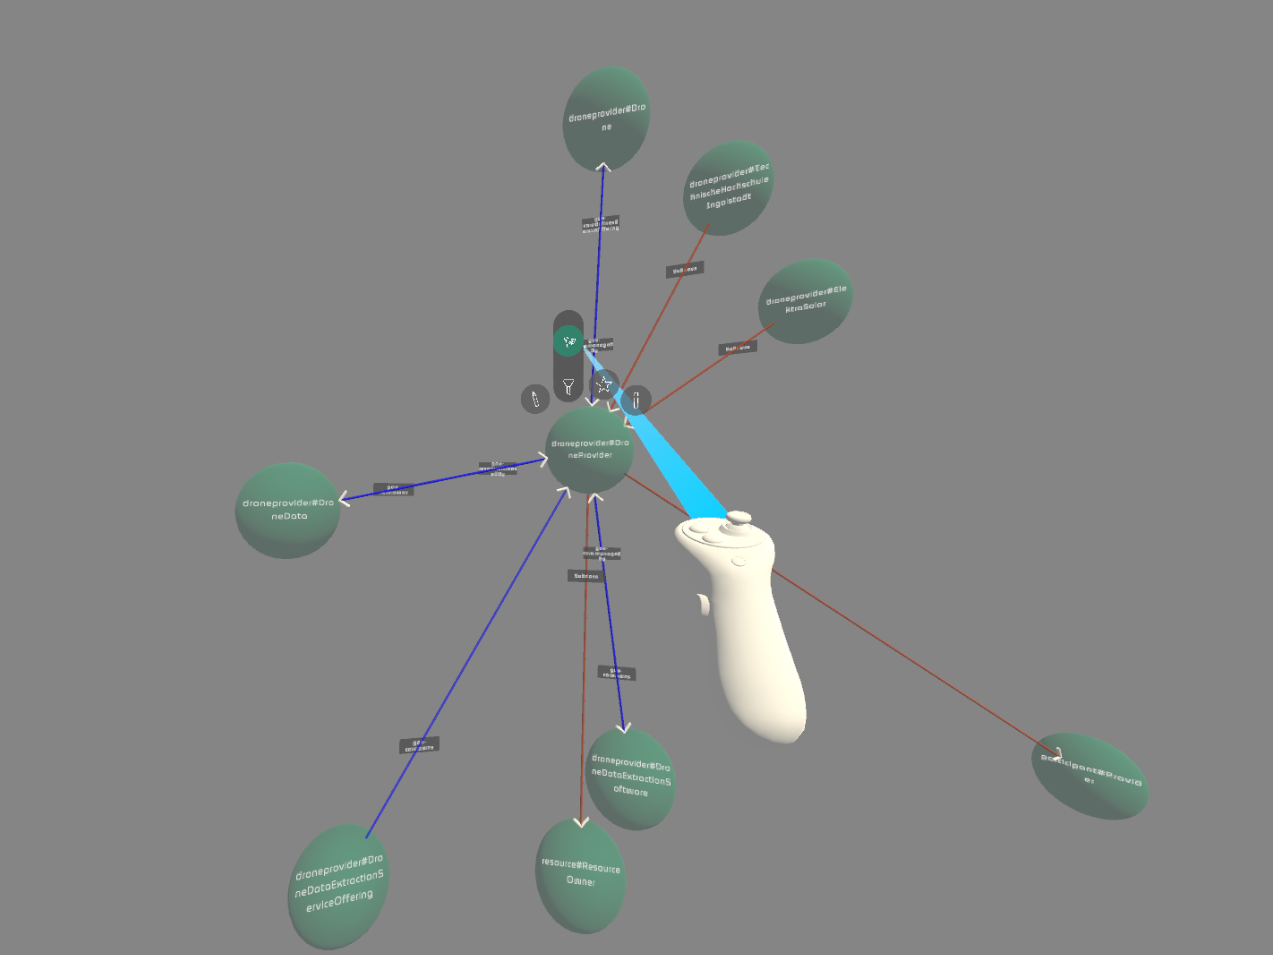
\includegraphics[width=\textwidth]{chapter2/figures/postfilter.png}
       \caption{Fragmento de escena después de filtrar}
   \end{subfigure}
  \caption{Filtrar por conexiones}
\end{figure}

En múltiples entrevistas y ensayos que hemos hecho con distintos participantes, hemos obtenido excelentes devoluciones sobre esta funcionalidad, incluso con ideas para mejorarla.

\subsection{Resaltar burbuja}

En caso que queramos distinguir una burbuja específica, podemos resaltarla con una herramienta que se encarga de cambiarle el color a su mesh y al de sus conectores. Gracias a esto, podemos identificarla fácilmente dentro de la red de nodos y conexiones por más compleja o compacta que sea.

\begin{figure}[ht]
   \begin{center}
      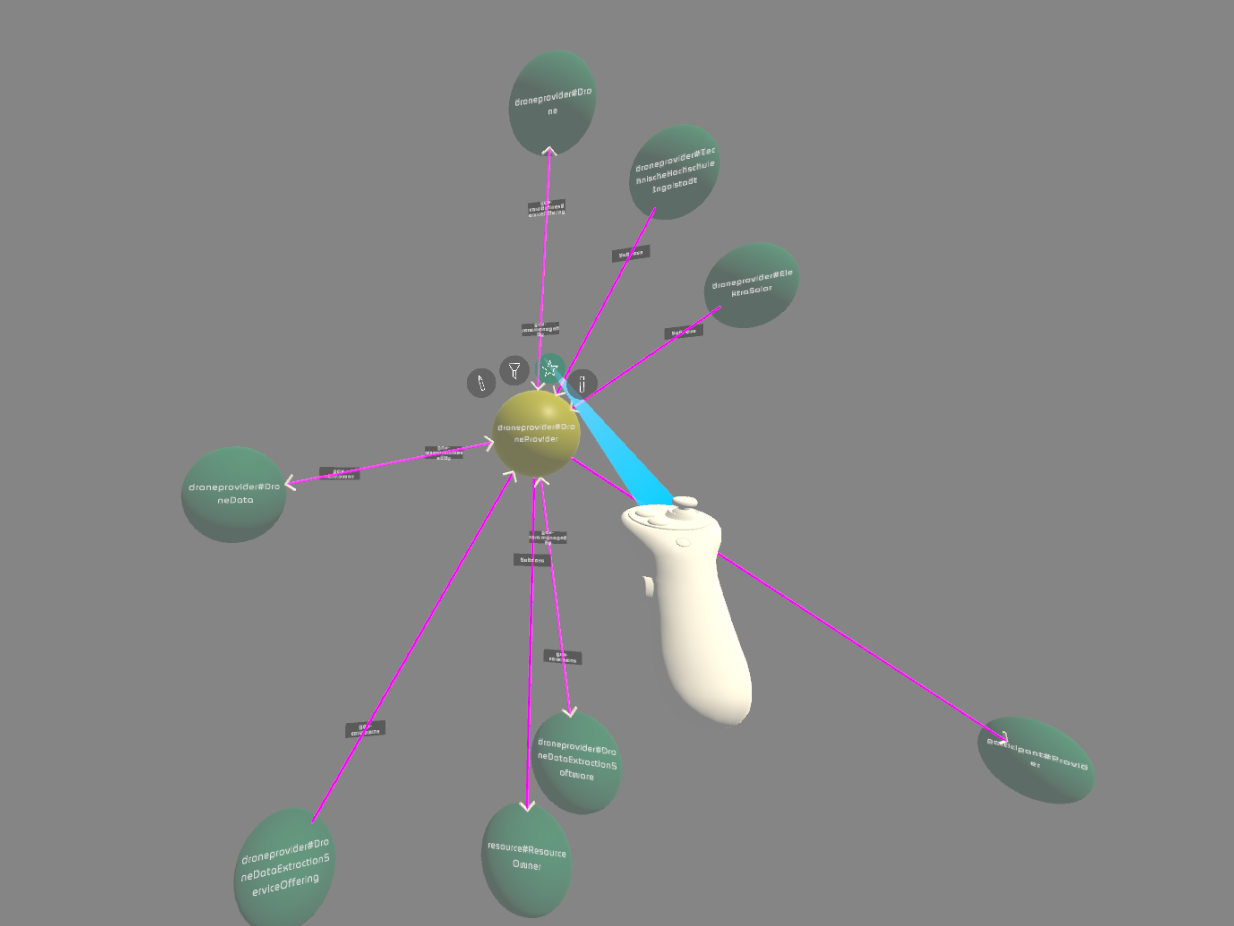
\includegraphics[width=0.55\linewidth]{chapter2/figures/highlight_tool.png}
   \end{center}
   \caption[Resaltar burbuja]
   {\footnotesize Resaltar burbuja}
\end{figure}

\subsection{Panel de información}

Cada clase posee una lista con comentarios o propiedades que aclaran algún aspecto específico. Toda esta información la mostramos en un panel que pertenece a cada burbuja.

\begin{figure}[ht]
   \begin{center}
      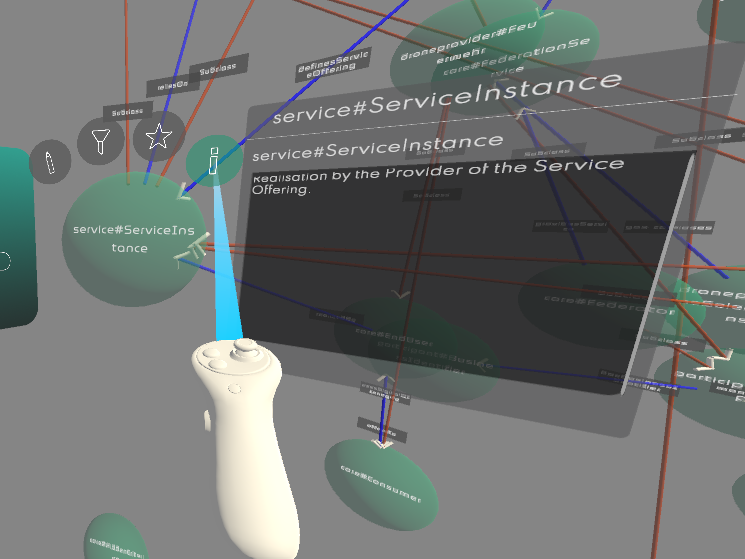
\includegraphics[width=0.55\linewidth]{chapter2/figures/informationPanel.png}
   \end{center}
   \caption[Panel de información]
   {\footnotesize Panel de información}
\end{figure}

\subsection{Herramientas de edición}

Si bien la edición excede el objetivo inicial de nuestro visualizador, también decidimos agregar algunas pocas herramientas para probarlas en algunos ensayos con participantes expertos en trabajo con ontologías y así obtener devoluciones que nos ayuden a planificar desarrollo futuro. En primera instancia, creamos los métodos para crear, eliminar y editar una burbuja (nombre y ontología a la que pertenece).

\begin{figure}[ht]
   \centering
   \begin{subfigure}{0.3\textwidth}
       \centering
       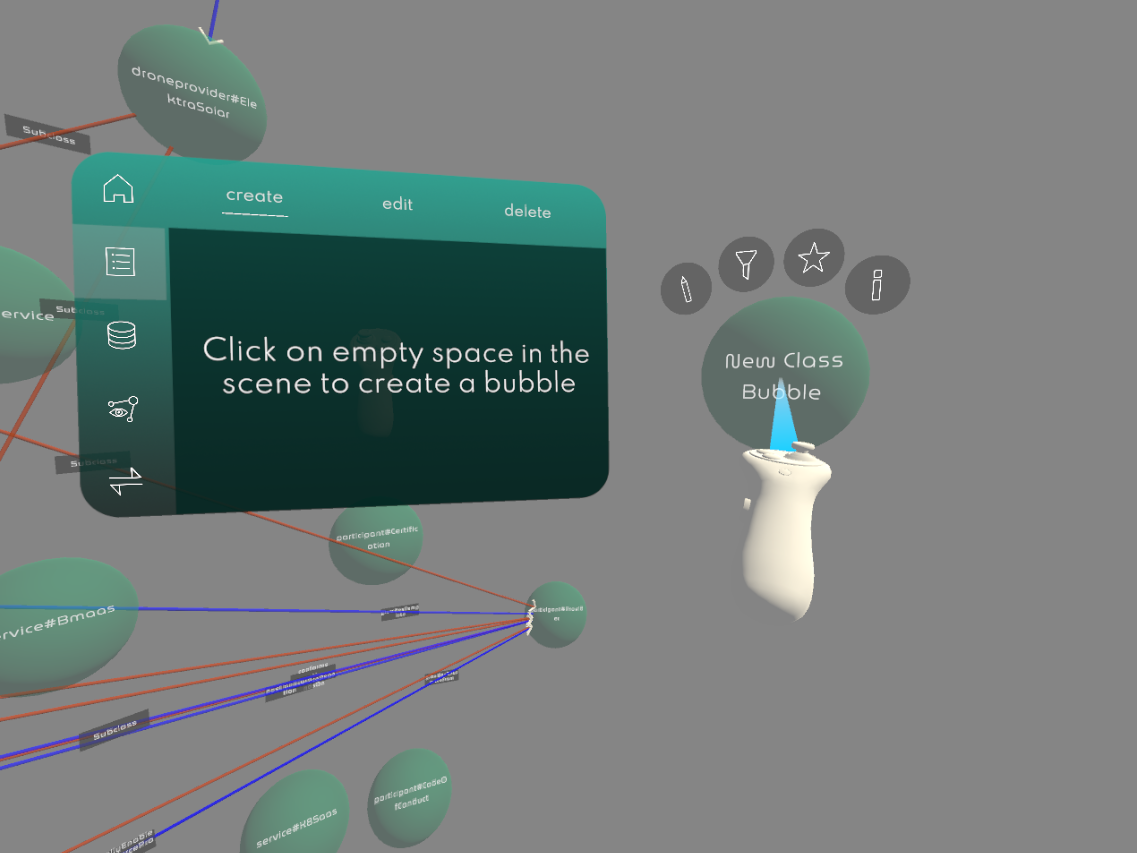
\includegraphics[width=\textwidth]{chapter2/figures/createbubble.png}
       \caption{Crear burbuja}
   \end{subfigure}
   \hfill
   \begin{subfigure}{0.3\textwidth}
       \centering
       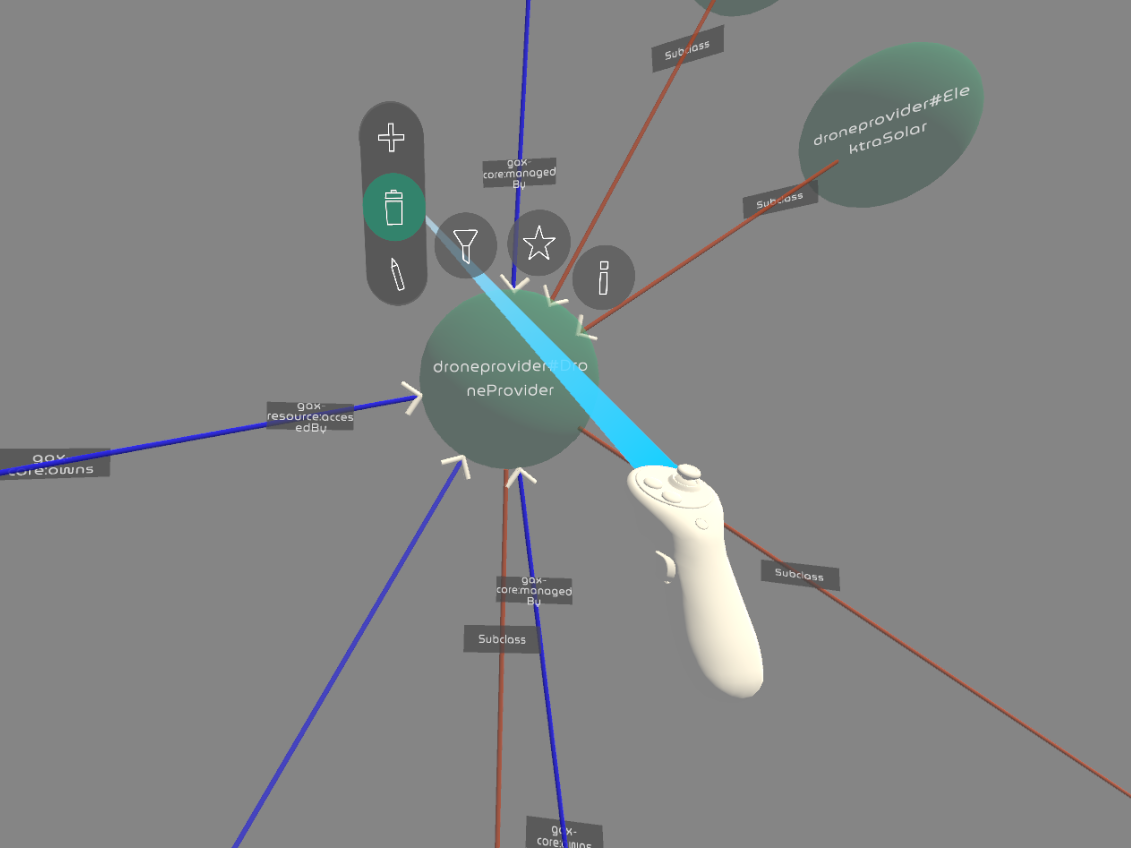
\includegraphics[width=\textwidth]{chapter2/figures/deletebubble.png}
       \caption{Eliminar burbuja}
   \end{subfigure}
   \hfill
   \begin{subfigure}{0.3\textwidth}
       \centering
       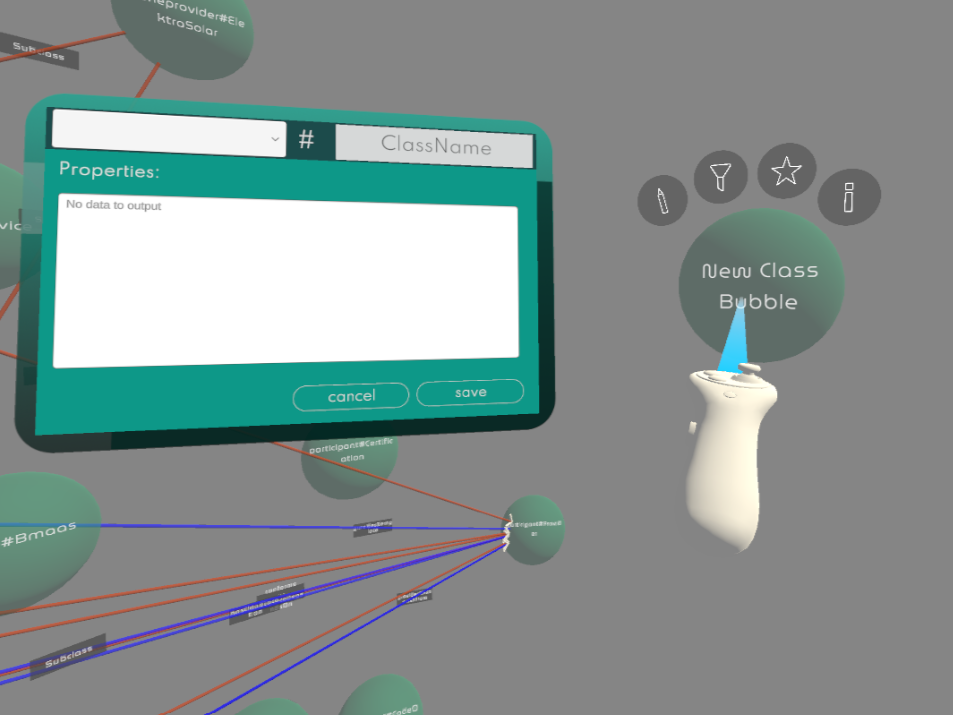
\includegraphics[width=\textwidth]{chapter2/figures/editbubble.png}
       \caption{Editar burbuja}
   \end{subfigure}
  \caption{Herramientas de edición}
\end{figure}

\section{Funciones Desarrolladas}

\subsection{Sistema de Búsqueda}

Implementar un sistema de búsqueda es casi obligatorio a la hora de crear un software de datos e información. Siempre necesitamos comprobar la existencia de clases y en la mayoría de los casos los resultados de búsqueda tienen también una funcionalidad asociada. En nuestro caso optamos por 2 diferentes, que pueden ser habilitadas desde el inspector de Unity: resaltar la burbuja elegida o teletransportarse a ella si se desea. Esto demostró ser extremadamente útil y escala muy bien si la cantidad de clases aumenta.

Para el ingreso de texto de búsqueda, primero optamos por utilizar un teclado virtual importado de Github que acoplamos al menú del controlador \cite[]{Keyboard}. Así podemos seleccionar con el puntero de la mano derecha cada letra que queramos buscar. 

El proceso de búsqueda es manejado por el \textit{Search Manager} y su método \textit{Search()} se ejecuta cada vez que se lance la función de callback \textit{On Value Changed} del campo de entrada de texto del buscador. Este objeto contiene una lista \textit{List<GameObject>Elements} que contiene referencias a todas las clases de la escena.

Cuando hay una coincidencia entre el texto de entrada y el nombre de cualquier burbuja, creamos botones dentro de un panel y los referenciamos a su burbuja correspondiente, de modo que podemos llamar a un método específico al pulsar sobre él. Si no hay coincidencia alguna, habilitamos un objeto que muestra un mensaje al usuario, indicándole que no hay resultado para la búsqueda realizada. Para esto utilizamos el booleano \textit{flagFoundObjects} para determinar los diferentes casos posibles de la búsqueda.

Es importante aclarar que cada vez que ingresamos un caracter en el buscador, debemos resetear los resultados anteriores, ya que estamos acotando la cantidad de resultados posibles. Esto significa que al principio del método de callback, primero debemos vaciar las listas de resultados y sus correspondientes botones instanciados. Todo esto lo podemos ver en el siguiente extracto de código.

\lstinputlisting[caption={Método Search()}, label=lst:csharp, linerange={66-92}]{appendix/codes/SearchScript.cs}

Los métodos utilizados son los siguientes:
\begin{itemize}
   \item Search: este es el método de callback cada vez que se modifica el campo de entrada de texto. Se encarga de comparar el texto ingresado con los nombres de las clases de la escena y crear una lista de resultados compuesta por referencias a las burbujas correspondientes.
   \item DeleteButtons: cada vez que ingresamos una letra, los resultados cambian. Por esta razón, debemos borrar los botones de los resultados de la búsqueda anterior.
   \item CreateButtons: instancia un botón por cada burbuja que haya dentro de la lista de resultados y realiza las conexiones necesarias para las funciones de callback de cada botón, ya se teletransportar o resaltar.
   \item ResetSearch: vacía el campo de entrada para cuando se complete una función de callback y así se resetea el sistema.
   \item UpdateResultsButton: es un sistema de \textit{flag} para determinar el mensaje de estado de búsqueda. Este es transmitido al usuario a través de un cuadro de texto.
\end{itemize}

Esta herramienta se incorpora al menú de la mano, que se acopla al mando de la mano izquierda en la simulación, e interactuamos con él con el raycast del mando de la mano derecha.
En la Figura 2.11 tenemos una captura de imagen del simulador que muestra como sería el resultado de buscar ``dro''. Dentro de lo encontrado, resaltamos cualquier parte del texto que coincida con la búsqueda, ya que hemos utilizado el método propio de los strings \textit{Contains()} para identificar coincidencias en cualquier parte del nombre de la clase.

\begin{figure}[ht]
   \begin{center}
      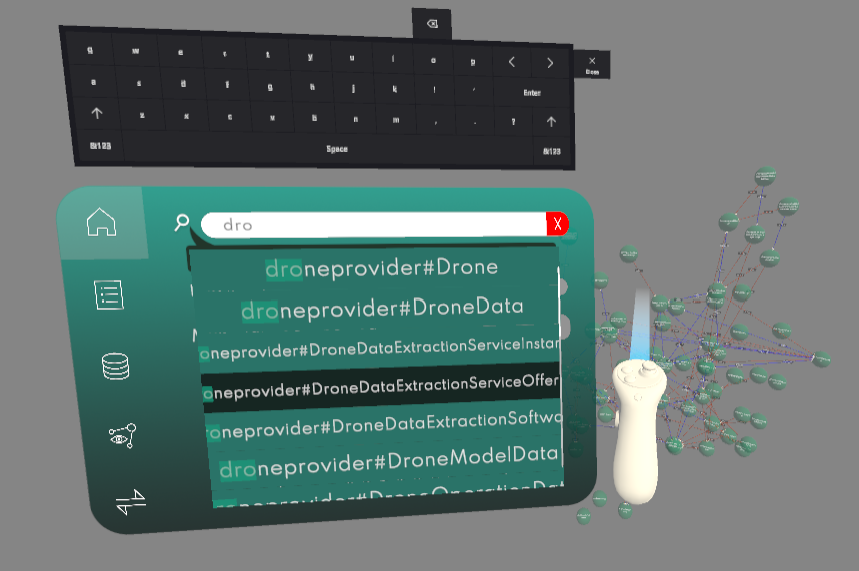
\includegraphics[width=0.7\linewidth]{chapter2/figures/searchtool.png}
   \end{center}
   \caption[Búsqueda de clases y resultados]
   {\footnotesize Búsqueda de clases y resultados}
\end{figure}

Al seleccionar alguno de los resultados, lanzaremos la función de callback que hayamos seleccionado en el inspector antes de darle Play al visualizador. Si hemos seleccionado el Resaltador, llamaremos al mismo método que está conectado al botón del menú de cada burbuja para cambiarle el color. Si decidimos utilizar la Teletransportación, debemos brindarle al botón del resultado toda la información correspondiente a la posición de la burbuja para iniciar un \textit{Teleport Request} hacia ella según el \textit{XR Interction Toolkit}.

\lstinputlisting[caption={Rutina de teletransportación}, label=lst:csharp, linerange={46-74}]{appendix/codes/TeleportOnSearch.cs}

\subsection{Sistema de Reconocimiento de Voz}

Para completar el Sistema de Búsqueda y proponer otra manera de ingresar texto al campo de búsqueda, pensamos que sería buena idea implementar un Mecanismo de Reconocimiento de Voz en tiempo real con IA para reducir los tiempos de tecleo. La principal limitación era que para conseguirlo necesitábamos una herramienta offline, de forma que el proyecto no dependiera de la conexión a internet y los datos se mantuvieran seguros y confidenciales.
Esto era bastante difícil dado que los mejores sistemas gratuitos de reconocimiento de voz requieren conexión o si no, son servicios pagos.

Después de investigar un poco encontré algunas alternativas, pero necesitaba probarlas y ver cuál funcionaba mejor.
\begin{itemize}
   \item \textbf{Servicios fuera de línea:}
   \begin{itemize}
      \item \textbf{DeepSpeech:}
      Motor Speech-To-Text de código abierto, que utiliza un modelo entrenado mediante técnicas de aprendizaje automático basado en el trabajo de investigación Deep Speech de Baidu. El proyecto no ha recibido actualizaciones desde 2020 y no hay soporte para las últimas versiones de Python, por lo que para usarlo es necesario utilizar una herramienta como win-pyenv para gestionar versiones antiguas. Siguiendo el único tutorial online, conseguí instalarlo pero el reconocimiento no fue bueno, alrededor de un 20\% y un 30\% de efectividad.
      \item \textbf{Vosk:}
      También es un kit de herramientas offline pero con soporte en diferentes idiomas. En su página web principal ofrecen un ejemplo de Unity, pero los resultados no fueron buenos y no se reconoció ninguna palabra.
      \item \textbf{Unity Keyword Recognizer:}
      Haciendo uso del servicio de reconocimiento de voz de Windows, podemos reconocer palabras y compararlas con comandos de la lista para activar eventos específicos. Inconveniente: hay que añadir manualmente cada comando a la lista y la llamada de retorno correspondiente.
      \item \textbf{WhisperAI:}
      Normalmente WhisperAI requiere una API y pagas cada vez que lo usas, pero también puedes instalarlo localmente usando la librería pip para Python.
      \item \textbf{Undertone:}
      Un activo de pago en Unity Store que también funciona sin conexión con WhisperAI.   \end{itemize}
   \item \textbf{Servicios en línea:}
   \begin{itemize}
      \item \textbf{Unity Dictation Recognizer:}
      Funciona igual que el Keyword Recognizer pero para identificar frases aleatorias necesitamos conexión a internet. Funciona bastante bien y reconoce los idiomas añadidos en la configuración de Windows del PC.
      \item \textbf{Hugging Face:}
      Es una IA online gratuita que proporciona una API con Unity y se encarga del reconocimiento de voz.
      \item \textbf{Recognissimo:}
      Es un activo de pago de Unity que también se encarga del reconocimiento de voz. Técnicamente está basado en el sistema Vosk.
   \end{itemize}
\end{itemize}

Habiéndolo consultado con mi equipo y mi supervisor, decidimos que implementaríamos la versión offline de WhisperAI y también probaríamos el Dictation Recognizer de Unity, dado que depende de Unity y Windows y usar la conexión a internet para eso era aceptable.
El sistema de búsqueda funciona de la misma manera, sólo estamos cambiando el método de entrada.

DictationRecognizer escucha la entrada de voz durante un período determinado y devuelve el resultado del reconocimiento, si es que hay \cite[]{DicationRecognizer}. En caso de superarse el tiempo límite de escucha o si se corta la conexión, actualizaremos el valor del flag correspondiente para comunicárselo al usuario con el cuadro de mensaje del buscador.

Los usuarios pueden registrarse y escuchar los eventos de hipótesis y frase completada. Los métodos Start() y Stop() activan y desactivan respectivamente el reconocimiento del dictado. Una vez que se ha terminado con el reconocedor, debe ser desechado utilizando el método Dispose() para liberar los recursos que utiliza. Liberará estos recursos automáticamente durante la recolección de basura con un coste adicional de rendimiento si no se liberan antes.

\lstinputlisting[caption={Start y Stop Dictation Recognizer}, label=lst:csharp, linerange={112-152}]{appendix/codes/DictationEngine.cs}

Por otro lado, la versión offline de WhisperAI fue muy interesante de usar ya que sólo puede leer archivos de audio y no voz en tiempo real \cite[]{WhisperAI}. Esto añadía un nuevo paso en el proceso de reconocimiento ya que primero teníamos que grabar la voz y luego interpretarla con la librería instalada.
Desarrollé un script en Python que era llamado desde Unity cuando queríamos buscar algo por voz, y primero registraría la voz en un archivo, luego reconocería el texto en él y lo enviaría de vuelta a Unity abriendo un proceso e imprimiendo en él.
Unity estaría escuchando cualquier dato de entrada del proceso abierto después de llamar al script de Python. Dado que ahora contamos con un lapso de tiempo de grabación de sonido y luego un tiempo de reconocimiento, fue necesario aumentar los valores posibles del flag que utilizamos para modificar el mensaje del cuadro de texto de estado de búsqueda. El mecanismo desarrollado indica al usuario través de un temporizador en qué momento hablar y que espere el procesamiento del audio cuando termine de grabar.

Para controlar el tiempo de procesamiento de audio, podemos seleccionar el tamaño del modelo de WhisperAI en inglés, por lo que podemos optimizar recursos u optar por un mejor reconocimiento según se prefiera.

\begin{figure}[ht]
   \begin{center}
      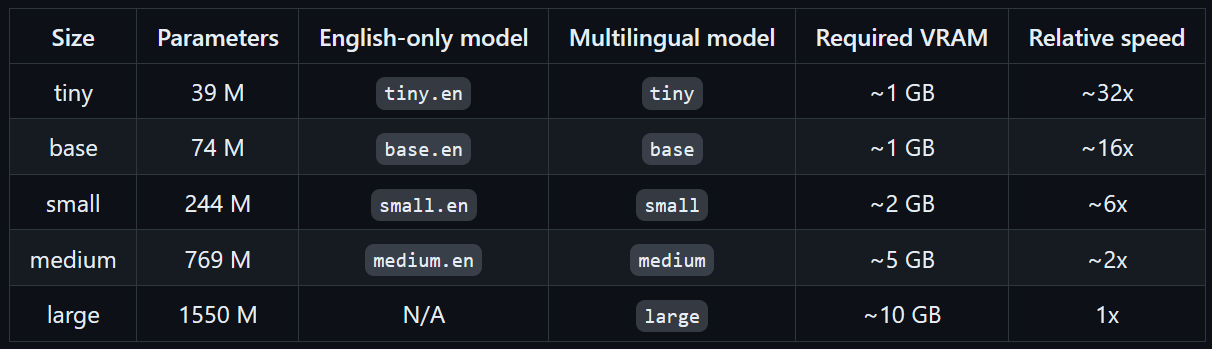
\includegraphics[width=0.85\linewidth]{chapter2/figures/whisperai.png}
   \end{center}
   \caption[Modelos de entrenamiento de Whisper AI]
   {\footnotesize Modelos de entrenamiento de Whisper AI}
\end{figure}

El código siguiente muestra la rutina de registro de audio junto con la interpretación con WhisperAI y la apertura del proceso de comunicación.

\lstinputlisting[caption={Registro de Audio y reconocimiento con WhisperAI}, label=lst:python, linerange={21-54}]{appendix/codes/recognition.py}

La incorporación del Reconocimiento de Voz nos deja un esquema de funcionamiento como el siguiente. El SearchManager recibe texto por teclado o por voz y actualiza los resultados de la búsqueda.

\begin{figure}[ht]
   \begin{center}
      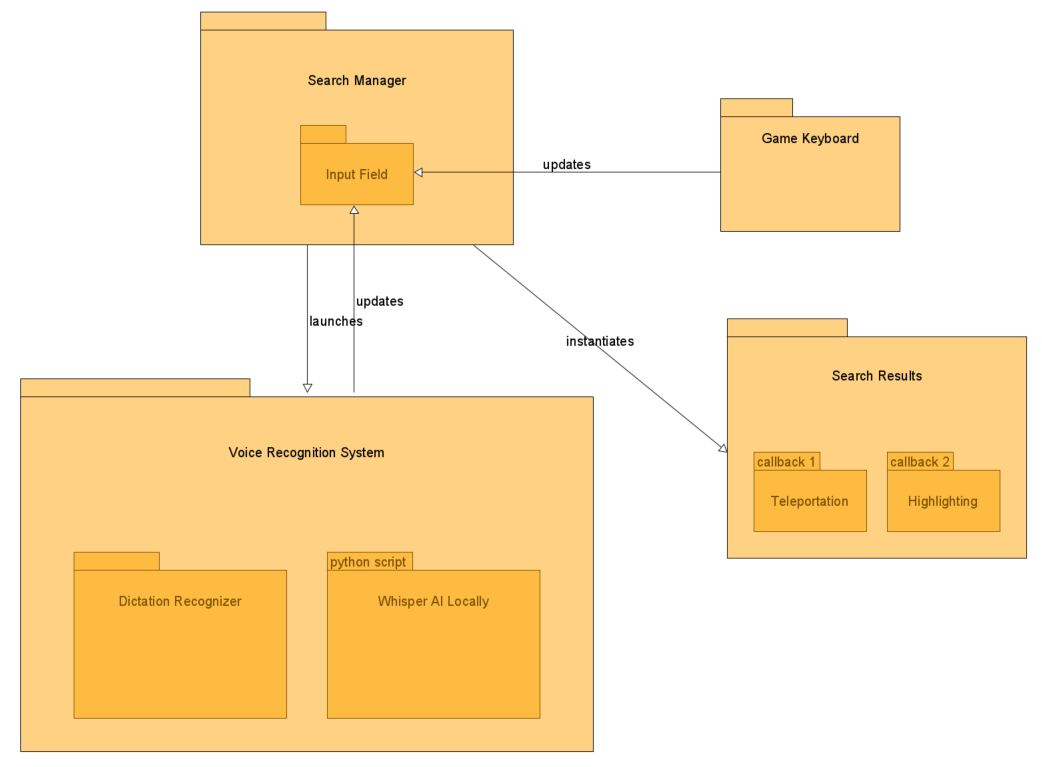
\includegraphics[width=1\linewidth]{chapter2/figures/searchsystem.png}
   \end{center}
   \caption[Diagrama de Paquetes del Sistema de Búsqueda]
   {\footnotesize Diagrama de Paquetes del Sistema de Búsqueda}
\end{figure}

\subsection{Menú Jerárquico}

Esta característica fue desarrollada al principio de mi pasantía y en ese momento las ontologías eran diferentes a las que estamos usando ahora, por lo que esta desactualizada y requiere ser reestructurada para ser agregada al formato actual del proyecto.

La idea era tener una pestaña en el menú de mano donde pudiéramos ver rápidamente qué clases había en la escena según su nivel en la ontología. La inspiración para esto fue la interfaz del sistema de carpetas del Explorador de Windows. Vemos una carpeta y, al hacer click en ella, expandimos el contenido que hay dentro y vemos las subcarpetas.
Así podemos navegar por nuestro sistema de datos y explorar todo lo que hay dentro. Esto era muy similar a nuestra antigua estructura ontológica, ya que teníamos un objeto Raíz y a partir de él empezábamos a conectar clases, de forma que cada una de ellas estaba conectada de alguna manera a ese objeto raíz.
Esto significaba que podíamos hacer click y expandir una clase, para ver qué clases derivaban de ella, según su nivel en la ontología. En la Figura 2.8, podemos ver una ilustración de como sería este funcionamiento.

\begin{figure}[ht]
   \begin{center}
      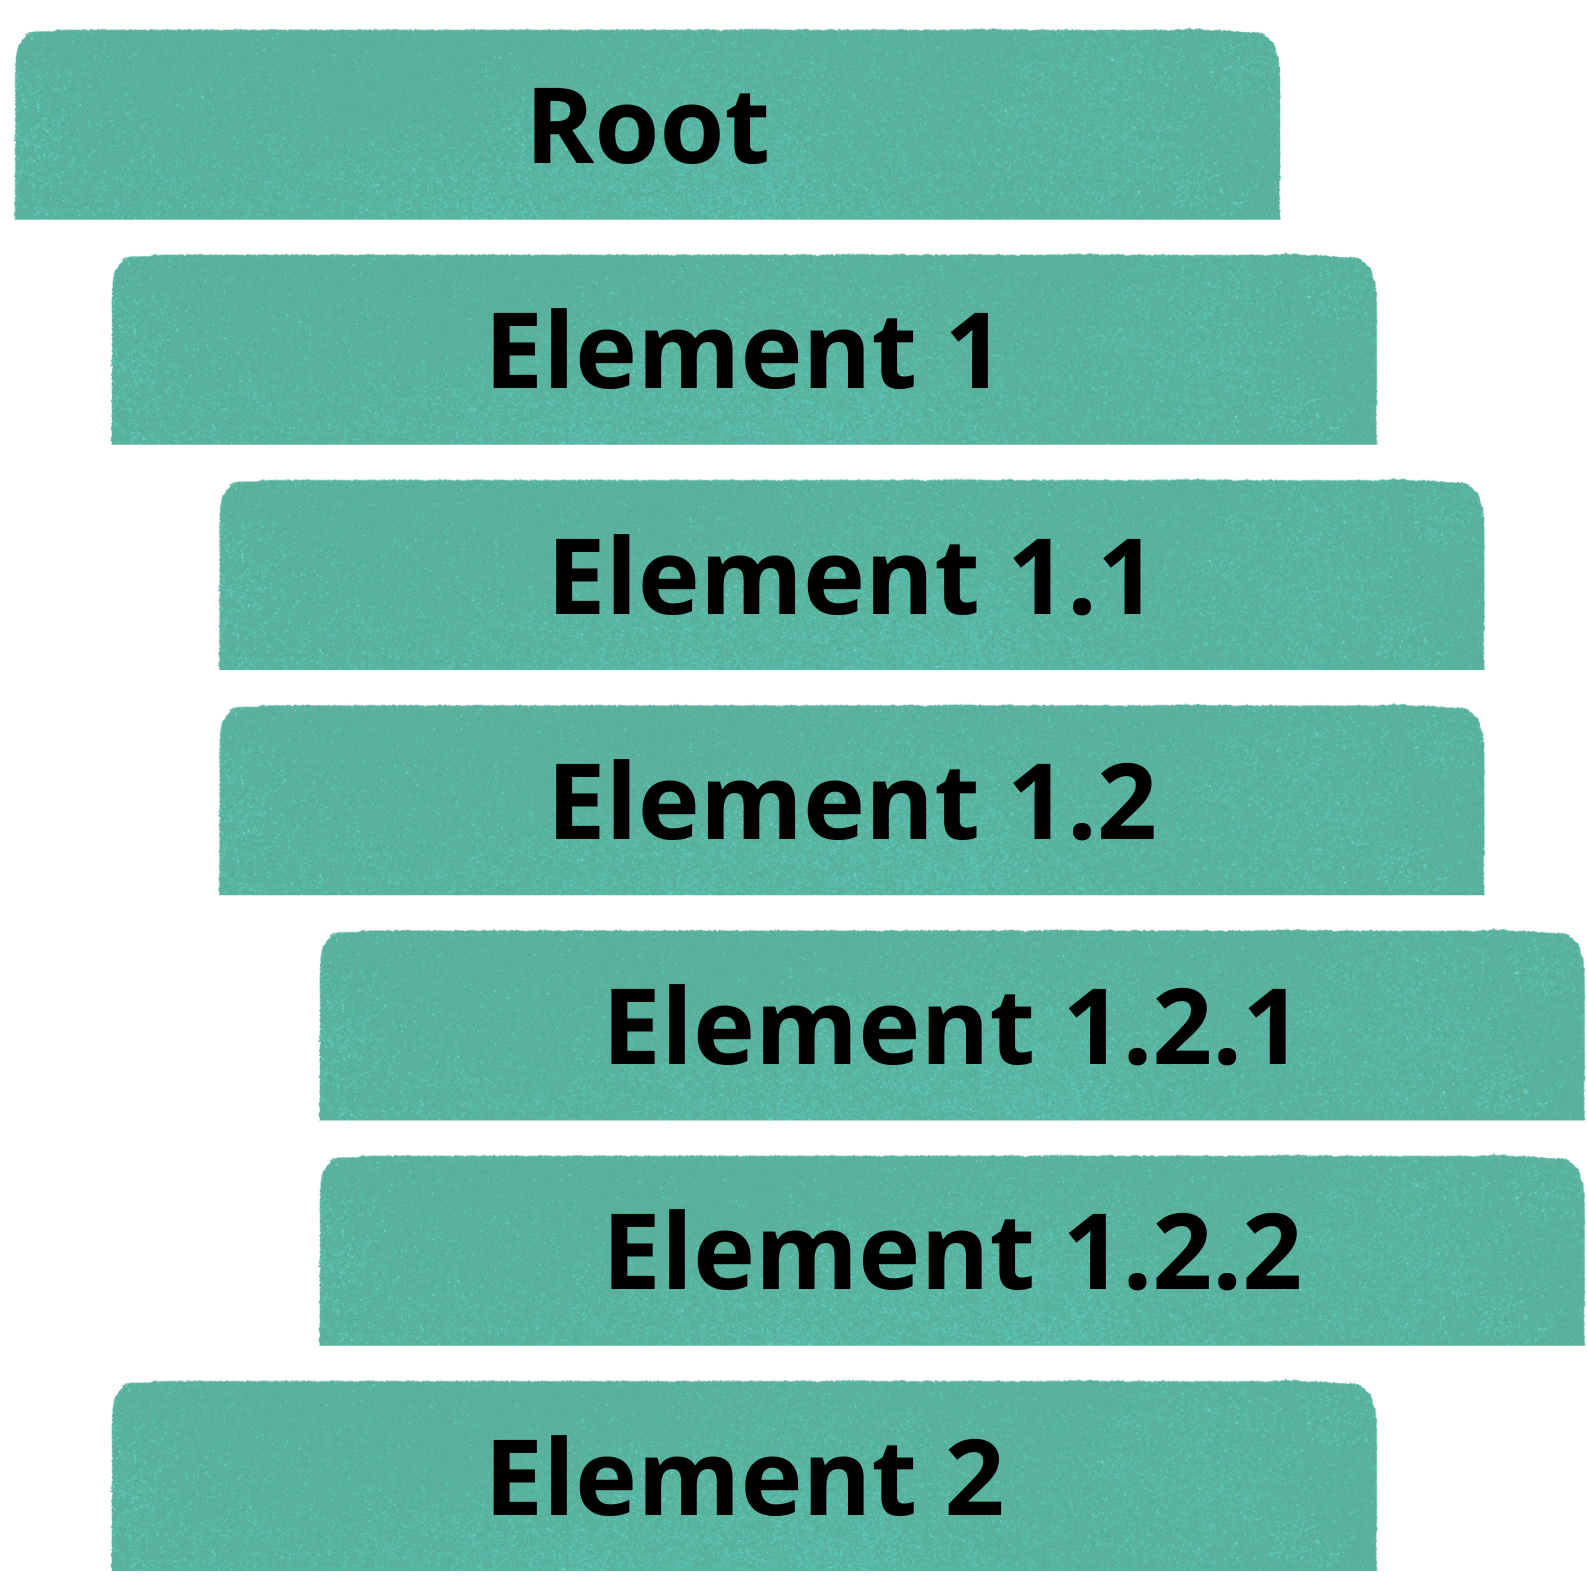
\includegraphics[width=0.6\linewidth]{chapter2/figures/hierarchy.png}
   \end{center}
   \caption[Ilustración gráfica de funcionamiento]
   {\footnotesize Ilustración gráfica de funcionamiento}
\end{figure}

La herramienta estaba implementada y funcionaba correctamente, y cada botón del menú también hacía referencia a las burbujas correspondientes, por lo que también teníamos funcionalidades de resaltado/teletransportación asociadas a ellas. Todo esto cambió cuando empezamos a importar ontologías desde ficheros jsonld y el concepto de objeto raíz dejó de existir. Ahora contamos con múltiples ontologías en simultáneo y hay varias burbujas que no heredan de ninguna otra.

\subsection{Importación desde archivos Jsonld}

Dado que no poseemos muchas herramientas de creación y edición de ontologías, salvo las pocas que he explicado, debemos tener una forma de importar datos de ontologías que hayan sido creadas por softwares externos. Luego de consultar con el equipo de Gaia-X, empezamos a planear el desarollo de una interfaz de importación de archivos de formato .jsonld.
El proceso de conversión es el resultado de un cuidadoso estudio por lo que necesita una explicación clara.

Dentro de nuestro simulador en Unity desarrollamos un sistema para guardar y cargar la información de todas las burbujas instanciadas en ese momento. Esto se realiza guardando en un archivo json la información básica de cada burbuja, como vimos en la sección 2.3, junto con los 3 valores (x,y,z) de la posición. Esto nos va a permitir cargar la información y reconstruir las ontologías en sesiones posteriores del visualizador. Podemos mover objetos y guardar la posición, sabiendo que el trabajo queda registrado y no se piede el progreso realizado.

Lo que nos falta es la conversión de datos entre los archivos descargados directamente de Gaia-X a nuestro tipo de archivo json que podemos leer y cargar en la escena. Para eso desarrollamos un objeto que al inicio de la escena, lee los archivos jsonld que le indiquemos y busca los datos necesarios para conformar un único archivo json que tendrá todas las clases que existan dentro de los archivos del ecosistema Gaia-X. La información que no haya sido utilizada para la importación, es conservada para el proceso de exportación cuando queramos recrear los archivos jsonld originales.

\begin{figure}[ht]
   \begin{center}
      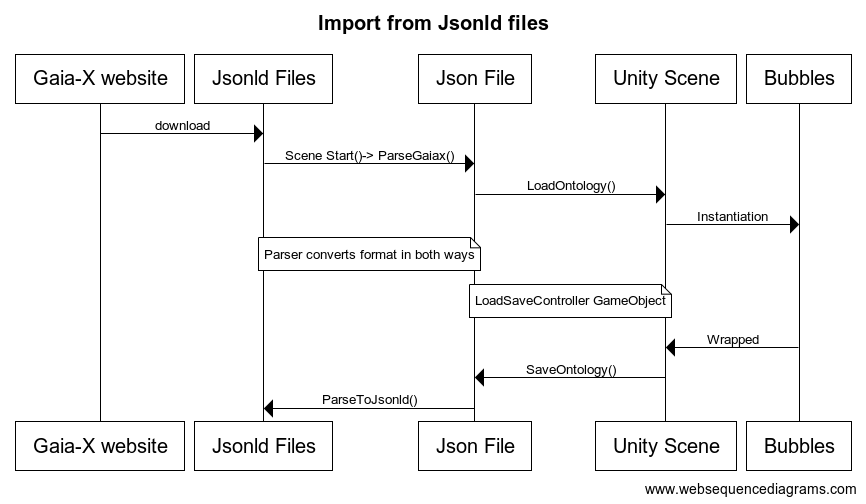
\includegraphics[width=0.9\linewidth]{chapter2/figures/import.png}
   \end{center}
   \caption[Diagrama de secuencia de importación de ontologías]
   {\footnotesize Diagrama de secuencia de importación de ontologías}
\end{figure}

La forma en que filtramos la información es con una secuencia de verificaciones de condición que comprueban la existencia de diferentes claves o propiedades json que nos guían y nos dicen qué información tomar y cuál dejar, ya que el fichero jsonld contiene mucho material que no vamos a utilizar en nuestra escena, pero que necesitamos conservar para cuando exportemos la escena.

A partir de los archivos jsonld que hemos descargado, buscamos en primer lugar objetos del tipo \textit{Class}, los cuales poseen el valor (``owl\#Class'') dentro de la propiedad \textit{type}. Con estos objetos podremos crear una lista con las burbujas a importar, asignarles un ID numérico, determinar a qué ontología pertenecen y un valor de posición, utilizando un archivo complementario. Estos datos son los que le dan identidad a cada burbuja individual, sin ninguna especificación de relaciones o conexiones con otras burbujas.

Los archivos que describen ontologías están enfocados en la información relacionada a las clases presentes junto con sus conexiones, por lo que no contiene indicaciones sobre la interepretación gráfica de la estructura. Esto significa que nosotros mismos debemos encontrar una manera de posicionar las burbujas dentro de la escena. Una forma sería desarrollar un algoritmo que determine valores de posición y busque optimizarlos según algún criterio como longitud de las conexiones, distribución de los objetos, espacio, etc. La otra opción consiste en utilizar una herramienta externa que se encarga de resolver este problema pero en dos dimensiones.
Lo que hacemos es, inmediatamente después de obtener los archivos de Gaia-X, cargarlos en este software y descargar el archivo con la información de la distribución gráfica. En el momento de instanciar clases en nuestro visualizador, accedemos a este último archivo y obtenemos los valores \textit{x} e \textit{y} de cada clase y asignamos un valor \textit{z} por defecto para darle la misma profundidad a todas las burbujas. Esto nos da como resultado una representación plana de la ontología dentro de nuestra escena 3D, pero ya hemos solucionado 2 de 3 valores de posición. El último lo resolveremos más tarde.

\lstinputlisting[caption={Búsqueda de información para la creación de clases}, label=lst:csharp, linerange={150-177}]{appendix/codes/Parser.cs}

Una vez tengamos una lista con todas las clases de los archivos a importar, podemos empezar a buscar conexiones entre ellas. Esto se hace buscando dentro de los mismos archivos, pero en este caso queremos encontrar objetos del tipo \textit{``owl\#ObjectProperty''} y todos aquellas clases que posean la propiedad \textit{``owl\#subClassOf''}, para encontrar ambos tipos de conexiones. Cada vez que encontremos cualquiera de estos casos, obtendremos de nuestra lista de clases las burbujas pertinentes e iremos completando la información faltante sobre sus conexiones.

Para entender mejor cómo funciona la herramienta de importación, será más fácil si utilizamos un ejemplo de conversión.

\begin{figure}[ht]
   \begin{center}
      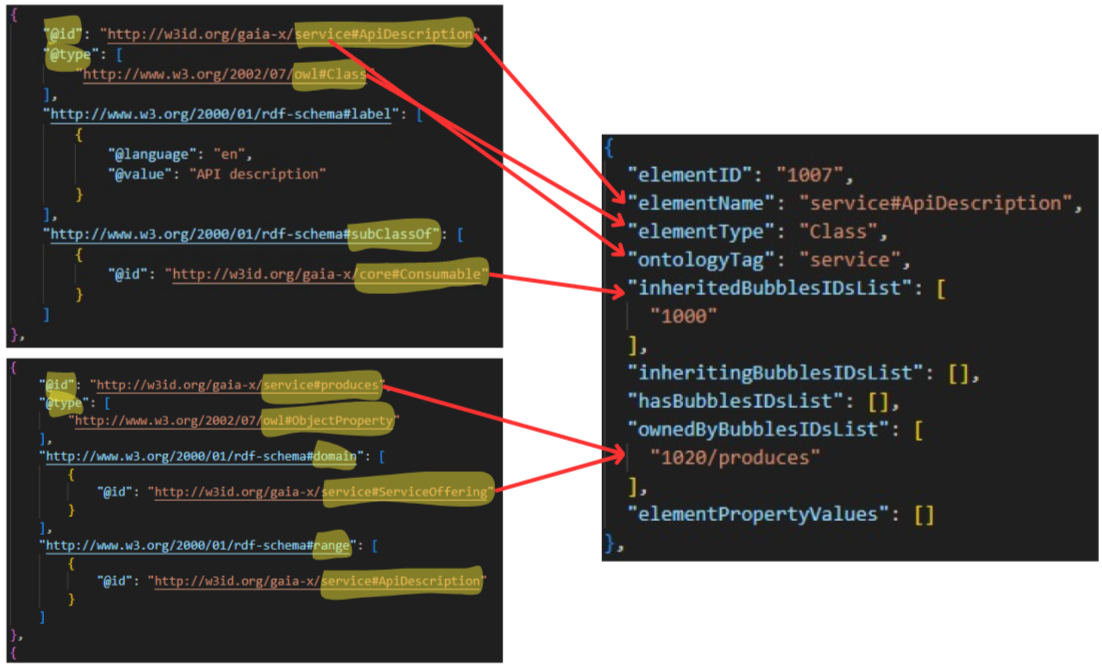
\includegraphics[width=0.9\linewidth]{chapter2/figures/parser.png}
   \end{center}
   \caption[Conversión de clase y conexión a formato interno]
   {\footnotesize Conversión de clase y conexión a formato interno}
\end{figure}

Gaia-X utiliza un estándar de información con identificadores web permanentes \cite[]{selfDescription} para mantener un nivel de comprensión, especificación y gobernanza en los datos. Esto se logra construyendo sobre la comprensibilidad universal asegurada por los estándares del \textit{World Wide Web Consortium} (W3C) \cite[]{w3id}.
Esto hace que gran parte del texto dentro de los archivos a importar sólo sirva dentro de este esquema de información, pero no es necesario utilizarlo en nuestra escena. Por esto, nuestro código se encarga principalmente de filtrar texto y conservar únicamente las porciones de \textit{string} que necesitemos. 

Cuando encontramos una clase, tenemos que deshacernos del URL en el id y quedarnos con el nombre real de la clase y la ontología a la que pertenece y asignarle un ID de objeto de juego único.
Para ello, nos fijamos en el id y el texto después del último separador ``/''. El caracter \# separará la etiqueta de la ontología a la izquierda y el nombre de la clase a la derecha.
Repetimos esta operación por cada objeto json de la lista hasta que hayamos guardado todos los objetos de tipo clase.

En el caso de las conexiones de subclase, simplemente tenemos que observar si las clases poseen una propiedad que indique la herencia (\textit{owl\#subClassOf}). Este campo nos señalará directamente la burbuja faltante para completar las listas de ambos extremos de la conexión.
Por otro lado, cada propiedad de objeto contiene información sobre el id de la conexión, el origen (dominio) y el destino (rango). Nuestra tarea consiste en buscar las burbujas especificadas en los extremos de la propiedad de objeto y agregarse mutuamente en las listas de conexión.

Así, por ejemplo, la conexión mostrada en la Figura 2.16 tiene el id de la conexión con dominio y rango. En este caso concreto, lo leeríamos así : "La clase \textit{Service Offering} de la ontología \textit{service} \textbf{produce} la clase \textit{ApiDescription} de la ontología \textit{service}". 
El URL subClassOf de la otra subfigura de la izquierda nos indicará de qué clase estamos heredando en este momento. En este caso, ``\textit{ApiDescription} de la ontología \textit{service} \textbf{hereda} de la clase \textit{Consumable} de la ontología \textit{core}''. Lo que hacemos ahora es añadir estas conexiones en las listas correspondientes con nuestro propio formato. La conexión de propiedad objeto se añade en la lista ``ownedByBubblesList'' con el id del origen (dominio) y su etiqueta. En el otro extremo, añadiremos el id del destino o rango (1007 en este caso) en la lista ``hasBubblesIDsList''. La conexión subClass
funciona de forma similar. Nuestra ApiDescription hereda de la burbuja 1000, que se añade a la ``inheritedBubblesList''.

\lstinputlisting[caption={Rutina de búsqueda de conexiones}, label=lst:csharp, linerange={296-324}]{appendix/codes/Parser.cs}

\begin{figure}[ht]
   \begin{center}
      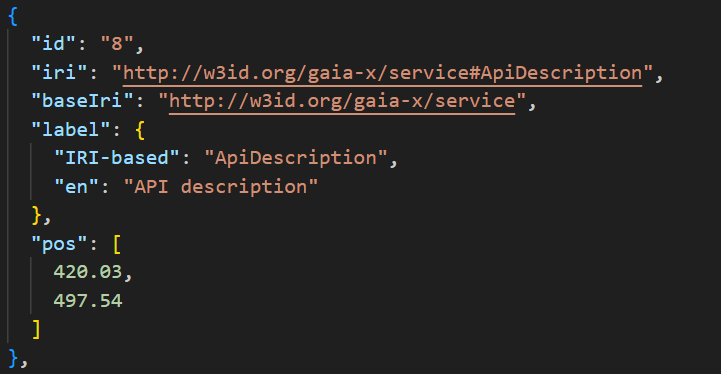
\includegraphics[width=0.7\linewidth]{chapter2/figures/position.png}
   \end{center}
   \caption[Objeto Json del archivo de posiciones]
   {\footnotesize Objeto Json del archivo de posiciones}
\end{figure}

La figura 2.17 muestra un objeto json de posición. Lo único que debemos hacer es buscar el id (url) de la clase en cuestión dentro del campo ``iri'' de los objetos json del archivo y recuperar los valores de la propiedad "pos".

\subsection{Exportación a archivos Jsonld}

El proceso de Exportación es muy similar, ya que leerá toda la información actual de cada burbuja en la escena y la guardará en un archivo json. Nuestro Parser tomará cada elemento y creará la clase Gaia-X correspondiente en un archivo jsonld. La lógica sigue siendo la misma, crear todas las clases y una vez que hayamos terminado, crear todas las conexiones. La única diferencia radica en que nuestro formato de guardar/cargar siempre especifica los mismos campos de propiedad dentro de cada objeto json, incluso si no contienen información. En cambio, los archivos de Gaia-X sólo especifican las propiedades que tengan un valor asociado. Para cumplir con el éstandar,
es necesario utilizar un Diccionario y especificar las propiedades y valores a través de las \textit{keys} del mismo. En el siguiente fragmento de código podemos ver esta implementación, donde \textit{dataToExport} es el nombre del diccionario que utilizamos.

\lstinputlisting[caption={Ejemplo de creación de llave en el Diccionario a exportar}, label=lst:csharp, linerange={596-605}]{appendix/codes/Parser.cs}

Esta herramienta de Importación/Exportación es crucial para el proyecto. Sin ella, no tendríamos la interoperabilidad necesaria. Pero para ello, debemos estar seguros de que no estamos perdiendo información en ningún paso o dirección del proceso. Esto significa que tenemos que comprobar todas las listas con frecuencia y buscar anomalías y datos irregulares.

Una vez que terminemos las principales tareas de visualización, podremos enfocarnos en tareas de edición y creación por lo que las ontologías sufrirán modificaciones dentro de nuestra aplicación y si esta herramienta funciona correctamente, deberíamos ver los resultados en los archivos exportados.

\subsection{Contenedores de Ontologías}

\begin{figure}[ht]
   \begin{center}
      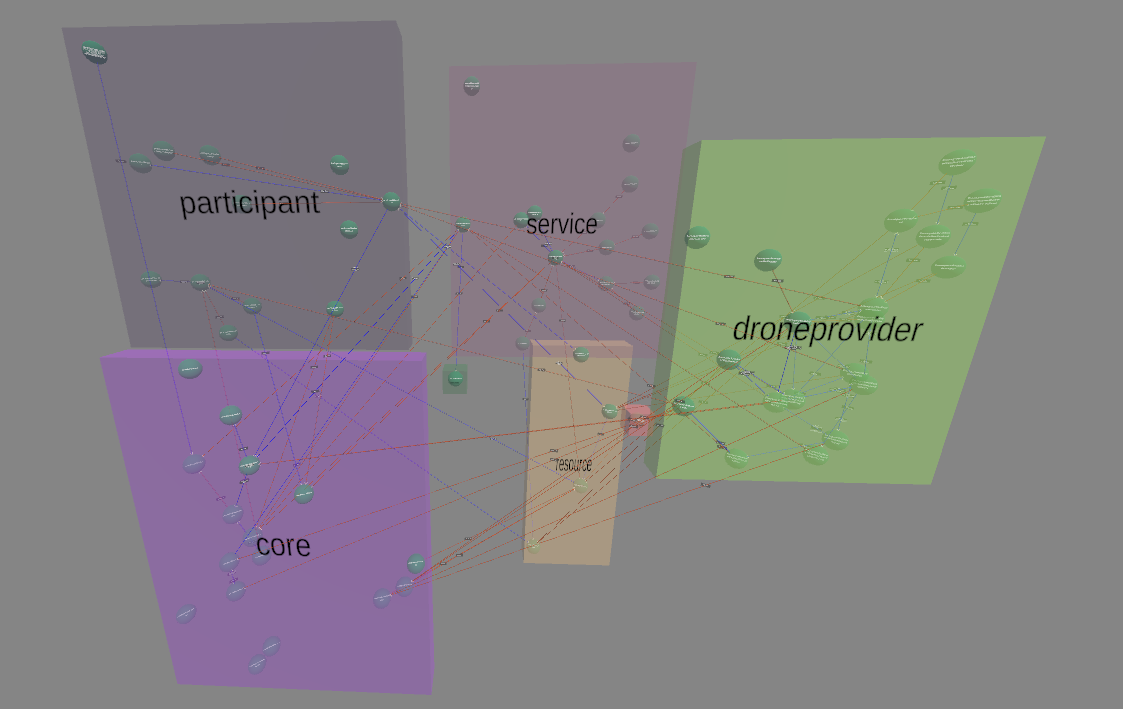
\includegraphics[width=0.8\linewidth]{chapter2/figures/ontologies&containers.png}
   \end{center}
   \caption[Ontologías y sus contenedores]
   {\footnotesize Ontologías y sus contenedores}
\end{figure}

La idea de esta característica es delimitar gráficamente cada ontología de manera que podamos diferenciarlas fácilmente. Además, cada contenedor debe ser interactivo para que uno pueda seleccionarlos y moverlos en el espacio, y al hacerlo, todas las clases contenidas se moveran dentro del bloque. Esto creará una nueva capa de interacción en nuestra simulación, permitiéndonos interactuar tanto con burbujas como con ontologías completas. A partir de aquí, podemos añadir nuevas características que también se aplican a todas las clases de una ontología.

El diagrama de clases de la Figura 2.19 nos muestra cómo están conectados los scripts en el código. OntologyManager se encarga de instanciar los prefabs y rellenar las listas correspondientes de cada uno de los subgestores. Entonces:

\begin{figure}[ht]
   \begin{center}
      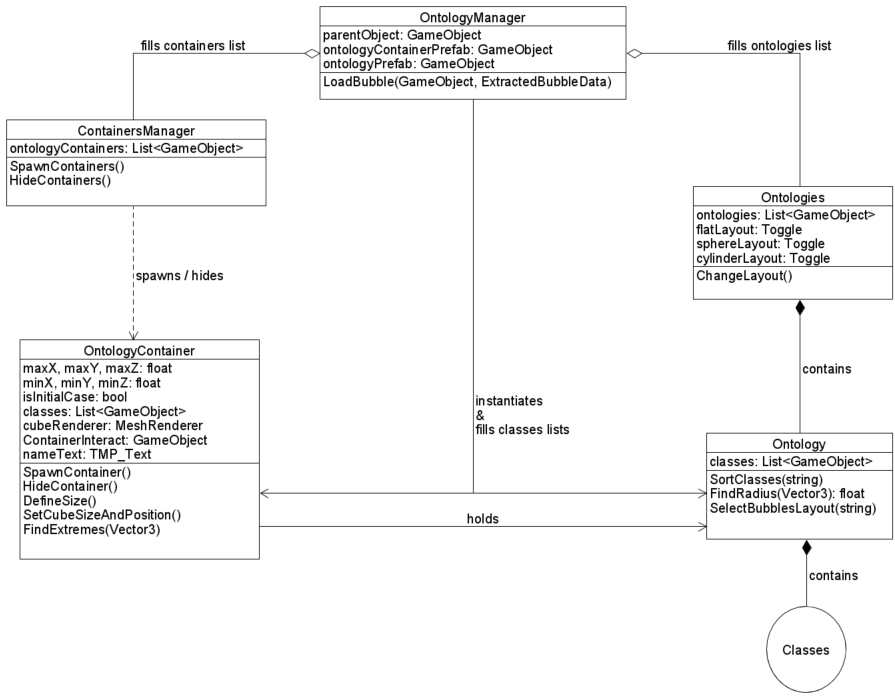
\includegraphics[width=1\linewidth]{chapter2/figures/containers_2.0.png}
   \end{center}
   \caption[Diagrama de clases para los contenedores]
   {\footnotesize Diagrama de clases para los contenedores}
\end{figure}

\begin{itemize}
   \item Todas las burbujas de una misma ontología están contenidas dentro del objeto padre \textit{Ontology}.
   \item Todas las ontologías están contenidas en un objeto padre mayor \textit{Ontologies}.
   \item Cada ontología tiene asociado un Container que va a encuadrar todas las burbujas correspondientes.
   \item El ContainersManager tiene referencias al Container de cada ontología.
\end{itemize}


Cada vez que creamos una nueva burbuja, debemos verificar si existe la ontología a la que pertenece. Si ya ha sido creada, tenemos que agregarla a la lista de burbujas. En caso contrario, debemos crear la ontología, asociarle un container, y agregar todos estos nuevos objetos a las listas correspondientes según la jerarquía. Podemos ver el siguiente fragmento de código para entender mejor los comandos. Esta secuencia la podemos ver en la Figura 2.20 más claramente.

\begin{figure}[ht]
   \begin{center}
      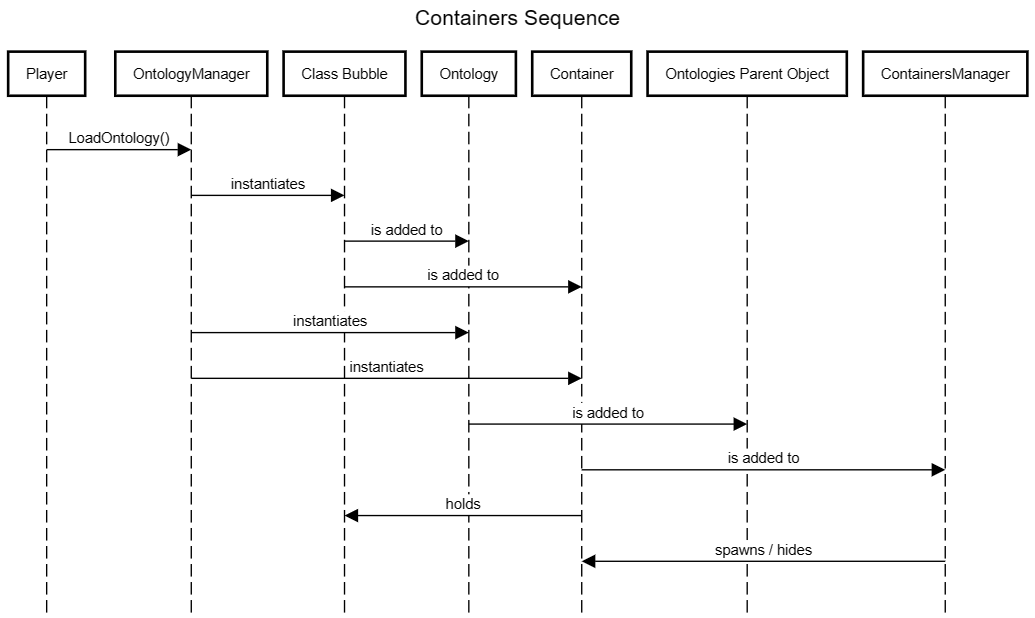
\includegraphics[width=1\linewidth]{chapter2/figures/container_sequence.png}
   \end{center}
   \caption[Diagrama de secuencia para la creación de clases y containers]
   {\footnotesize Diagrama de secuencia para la creación de clases y containers}
\end{figure}

\lstinputlisting[caption={Crear burbujas, ontologías y containers}, label=lst:csharp, linerange={282-310}]{appendix/codes/OntologyManager.cs}

ContainersManager.cs tiene el control de la funcionalidad, por lo que es el componente que necesitamos para los métodos de callback.

OntologyContainer.cs pertenece al objeto container y tiene los métodos de control respectivos para calcular su tamaño, posición y mostrarlo o esconderlo según sea requerido.

Cada contenedor también tiene un script VRInteractable para que podamos moverlo con el raycast de nuestro controlador. Lo bueno de esto es que cada clase contenida en él también se moverá en el mismo vector de desplazamiento y magnitud, por lo que todo se comportará como un bloque. Con esto conseguimos la capa de interacción mencionada anteriormente.

\subsection{Modos de distribución de ontologías}

Esta característica pretende complementar el proceso de importación, ya que estamos asignando un valor de tercera dimensión al vector de posición para instanciar la burbuja, pero todas tienen el mismo, por lo que estamos perdiendo el efecto 3D tan necesario. Para superarlo, vamos a utilizar formas geométricas básicas para describir cada ontología.
La idea consiste en determinar un objeto 3D con una forma específica, que englobe y contenga a las burbujas de cada ontología. Luego, utilizando la función del cuerpo que hayamos elegido, buscamos el valor \textit{z} para cada par \textit{x} e \textit{y} de cada burbuja. Esto va a generar una proyección de la ontología completa segun una curva deseada.

\lstinputlisting[caption={Ejemplo de forma cilíndrica}, label=lst:csharp, linerange={61-89}]{appendix/codes/Ontology.cs}

\begin{figure}[ht]
   \begin{center}
      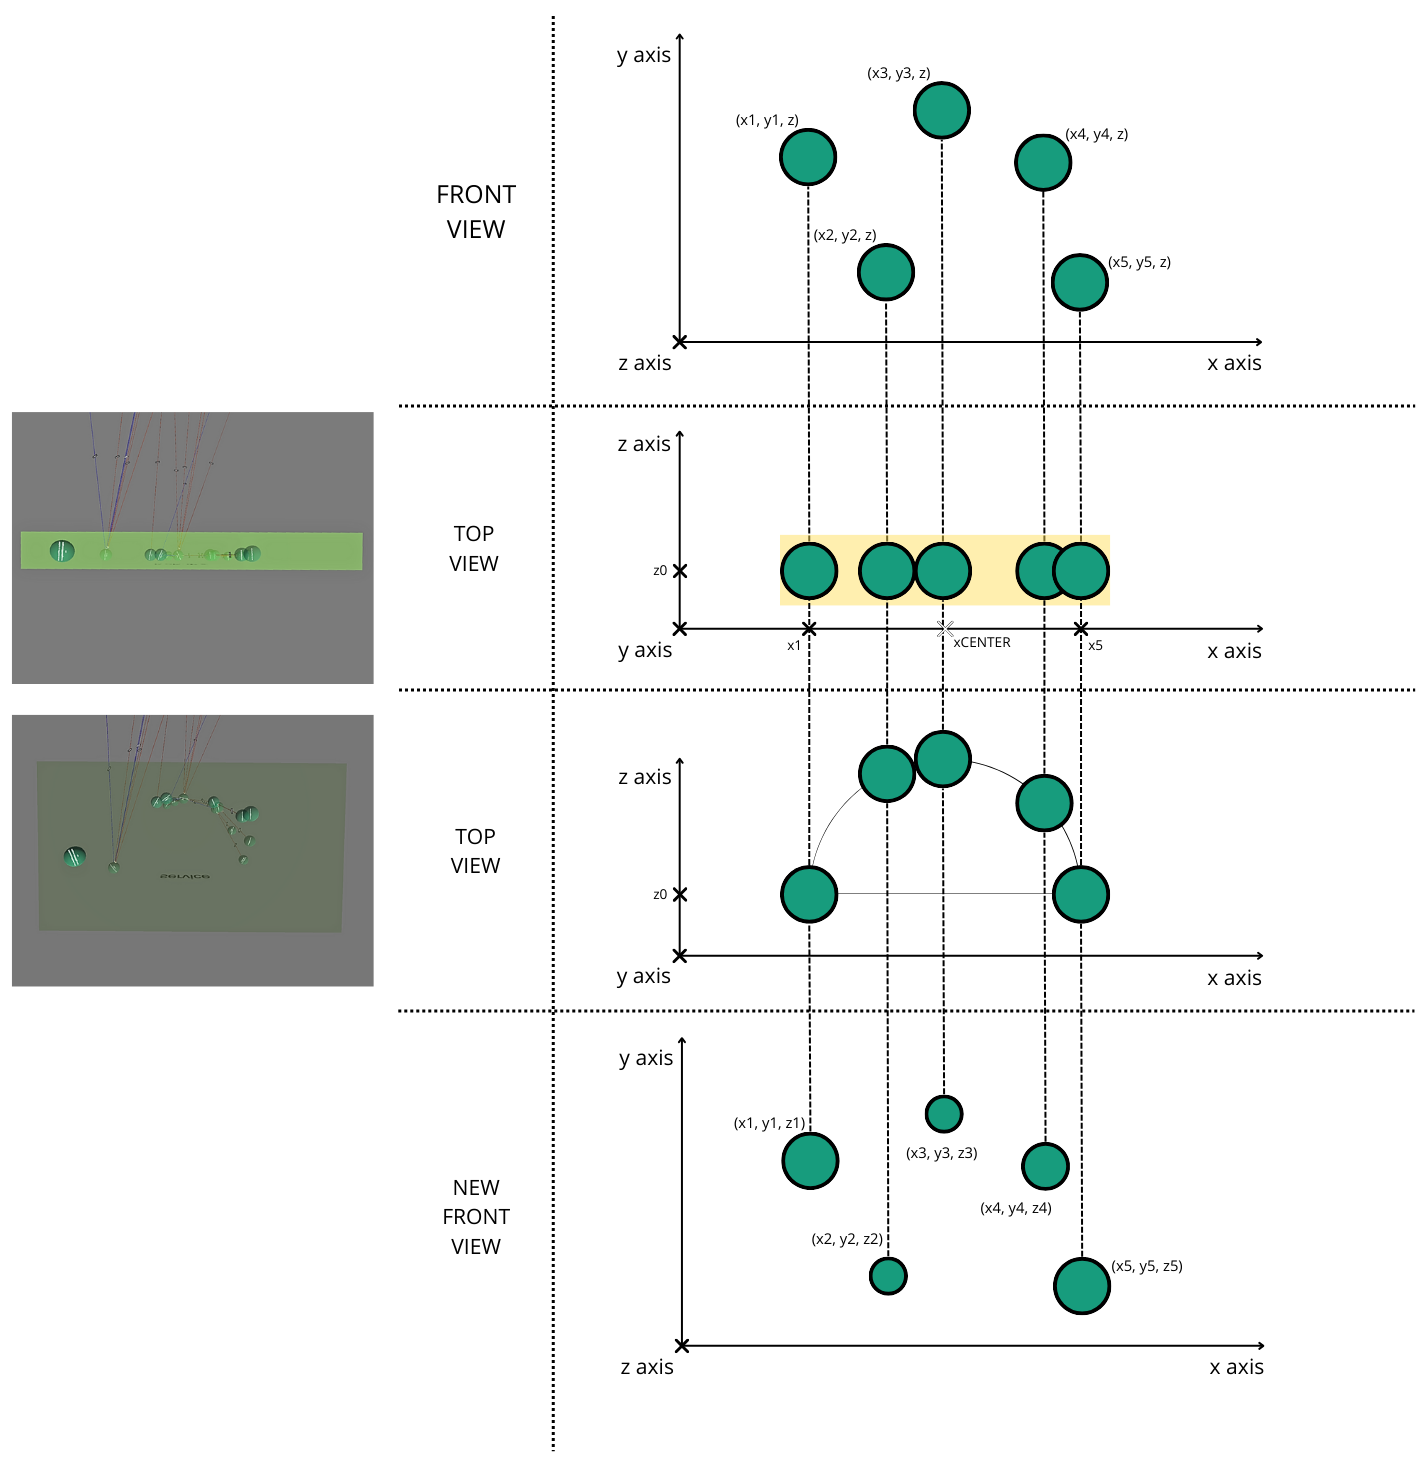
\includegraphics[width=1\linewidth]{chapter2/figures/clusters shape.png}
   \end{center}
   \caption[Cálculo de proyección para los modos de distribución]
   {\footnotesize Cálculo de proyección para los modos de distribución}
   \label{fig:mufigure17}
\end{figure}

En la Figura 2.21, vemos un esquema de cómo funciona el ejemplo anterior. Tomamos las burbujas de una ontología, calculamos la distancia x entre las más extremas y la utilizamos para crear un radio de cilindro. A continuación, colocamos cada burbuja en el valor z de este cilindro según las otras dos coordenadas a modo de proyección.
